\documentclass[a4paper,11pt]{book}
%\documentclass[a4paper,twoside,11pt,titlepage]{book}
\usepackage{listings}
\usepackage{float}

\usepackage{eurosym}

\usepackage{natbib}

\usepackage[utf8]{inputenc}
\usepackage[english]{babel}

\usepackage{pifont} %For ding marks, http://willbenton.com/wb-images/pifont.pdf
\usepackage{booktabs}
\usepackage{xcolor}

% \usepackage[style=list, number=none]{glossary} %
%\usepackage{titlesec}
%\usepackage{pailatino}


\usepackage{dcolumn}
\newcolumntype{.}{D{.}{\esperiod}{-1}}
\makeatletter
\addto\shorthandsspanish{\let\esperiod\es@period@code}
\makeatother


%\usepackage[chapter]{algorithm}
\RequirePackage{verbatim}
%\RequirePackage[Glenn]{fncychap}
\usepackage{fancyhdr}
\usepackage{graphicx}
\usepackage{afterpage}

\usepackage{longtable}

\usepackage{fancybox}

\usepackage[pdfborder={000}]{hyperref} %referencia


\usepackage{indentfirst}
%\usepackage[parfill]{parskip}

 %Own colors:
\definecolor{ownRed}{rgb}{0.858, 0.188, 0.478}
\definecolor{ownGreen}{rgb}{0.073, 0.532, 0.062}
\definecolor{ownOrange}{rgb}{0.6,0.6,0.0}

 %Own commands for own symbols:
\newcommand{\completeValue}{\textcolor{ownGreen}{\ding{51}}}
\newcommand{\noneValue}{\textcolor{ownRed}{\ding{55}}}
\newcommand{\partialValue}{\textcolor{ownOrange}{\ding{120}}}

% ********************************************************************
% Re-usable information
% ********************************************************************
\newcommand{\myTitle}{Título del proyecto\xspace}
\newcommand{\myDegree}{Grado en ...\xspace}
\newcommand{\myName}{Nombre Apllido1 Apellido2 (alumno)\xspace}
\newcommand{\myProf}{Nombre Apllido1 Apellido2 (tutor1)\xspace}
\newcommand{\myOtherProf}{Nombre Apllido1 Apellido2 (tutor2)\xspace}
%\newcommand{\mySupervisor}{Put name here\xspace}
\newcommand{\myFaculty}{Escuela Técnica Superior de Ingenierías Informática y de
Telecomunicación\xspace}
\newcommand{\myFacultyShort}{E.T.S. de Ingenierías Informática y de
Telecomunicación\xspace}
\newcommand{\myDepartment}{Departamento de ...\xspace}
\newcommand{\myUni}{\protect{Universidad de Granada}\xspace}
\newcommand{\myLocation}{Granada\xspace}
\newcommand{\myTime}{\today\xspace}
\newcommand{\myVersion}{Version 0.1\xspace}


\hypersetup{
pdfauthor = {\myName (email (en) ugr (punto) es)},
pdftitle = {\myTitle},
pdfsubject = {},
pdfkeywords = {palabra_clave1, palabra_clave2, palabra_clave3, ...},
pdfcreator = {LaTeX con el paquete ....},
pdfproducer = {pdflatex}
}

%\hyphenation{}


%\usepackage{doxygen/doxygen}
%\usepackage{pdfpages}
\usepackage{url}
\usepackage{colortbl,longtable}
\usepackage[stable]{footmisc}
%\usepackage{index}

%\makeindex
%\usepackage[style=long, cols=2,border=plain,toc=true,number=none]{glossary}
% \makeglossary

% Definición de comandos que me son tiles:
%\renewcommand{\indexname}{Índice alfabético}
%\renewcommand{\glossaryname}{Glosario}

\pagestyle{fancy}
\fancyhf{}
\fancyhead[LO]{\leftmark}
\fancyhead[RE]{\rightmark}
\fancyhead[RO,LE]{\textbf{\thepage}}
\renewcommand{\chaptermark}[1]{\markboth{\textbf{#1}}{}}
\renewcommand{\sectionmark}[1]{\markright{\textbf{\thesection. #1}}}
% Our own command to do a clear intro with a white line and
% avoid indent the next line as first in section and the
% justify of last line.
\newcommand{\intro}{\\ \\ \noindent}

\setlength{\headheight}{1.5\headheight}

\newcommand{\HRule}{\rule{\linewidth}{0.5mm}}
%Definimos los tipos teorema, ejemplo y definición podremos usar estos tipos
%simplemente poniendo \begin{teorema} \end{teorema} ...
\newtheorem{teorema}{Teorema}[chapter]
\newtheorem{ejemplo}{Ejemplo}[chapter]
\newtheorem{definicion}{Definición}[chapter]

\definecolor{gray97}{gray}{.97}
\definecolor{gray75}{gray}{.75}
\definecolor{gray45}{gray}{.45}
\definecolor{gray30}{gray}{.94}

\lstset{ frame=Ltb,
     framerule=0.5pt,
     aboveskip=0.5cm,
     framextopmargin=3pt,
     framexbottommargin=3pt,
     framexleftmargin=0.1cm,
     framesep=0pt,
     rulesep=.4pt,
     backgroundcolor=\color{gray97},
     rulesepcolor=\color{black},
     %
     stringstyle=\ttfamily,
     showstringspaces = false,
     basicstyle=\scriptsize\ttfamily,
     commentstyle=\color{gray45},
     keywordstyle=\bfseries,
     %
     numbers=left,
     numbersep=6pt,
     numberstyle=\tiny,
     numberfirstline = false,
     breaklines=true,
   }
 
% minimizar fragmentado de listados
\lstnewenvironment{listing}[1][]
   {\lstset{#1}\pagebreak[0]}{\pagebreak[0]}

\lstdefinestyle{CodigoC}
   {
	basicstyle=\scriptsize,
	frame=single,
	language=C,
	numbers=left
   }
\lstdefinestyle{CodigoC++}
   {
	basicstyle=\small,
	frame=single,
	backgroundcolor=\color{gray30},
	language=C++,
	numbers=left
   }

 
\lstdefinestyle{Consola}
   {basicstyle=\scriptsize\bf\ttfamily,
    backgroundcolor=\color{gray30},
    frame=single,
    numbers=none
   }


\newcommand{\bigrule}{\titlerule[0.5mm]}


%Para conseguir que en las páginas en blanco no ponga cabecerass
\makeatletter
\def\clearpage{%
  \ifvmode
    \ifnum \@dbltopnum =\m@ne
      \ifdim \pagetotal <\topskip
        \hbox{}
      \fi
    \fi
  \fi
  \newpage
  \thispagestyle{empty}
  \write\m@ne{}
  \vbox{}
  \penalty -\@Mi
}
\makeatother

\usepackage{pdfpages}
\begin{document}
\begin{titlepage}


\newlength{\centeroffset}
\setlength{\centeroffset}{-0.5\oddsidemargin}
\addtolength{\centeroffset}{0.5\evensidemargin}
\thispagestyle{empty}

\noindent\hspace*{\centeroffset}\begin{minipage}{\textwidth}

\centering

\includegraphics[width=0.9\textwidth]{img/logo_ugr.jpg}\\[1.4cm]

\textsc{ \Large FINAL DEGREE WORK \\[0.2cm]}
\textsc{ COMPUTER SCIENCE DEGREE }\\[1cm]
% Upper part of the page
%
% Title
{\Huge\bfseries SMS\\
}
\noindent\rule[-1ex]{\textwidth}{3pt}\\[3.5ex]
{\large\bfseries A proccesses acelerator for educational centers.}
\end{minipage}

\vspace{2.5cm}
\noindent\hspace*{\centeroffset}\begin{minipage}{\textwidth}
\centering

\textbf{Author}\\ {juan Antonio Fernández Sánchez}\\[2.5ex]
\textbf{Directores}\\
{Juan Julian Merelo Cuervos}\\[2cm]

\includegraphics[width=0.3\textwidth]{img/etsiit_logo.png}\\[0.1cm]
\textsc{Escuela Técnica Superior de Ingenierías Informática y de Telecomunicación}\\
\textsc{---}\\
Granada, Junio de 2017
\end{minipage}
%\addtolength{\textwidth}{\centeroffset}
%\vspace{\stretch{2}}
\end{titlepage}

\chapter*{}
%\thispagestyle{empty}
%\cleardoublepage

%\thispagestyle{empty}




\cleardoublepage
\thispagestyle{empty}

\begin{center}
{\large\bfseries SMS: A proccesses acelerator for educational centers}\\
\end{center}
\begin{center}
Juan Antonio Fernández Sánchez\\
\end{center}

%\vspace{0.7cm}
\noindent{\textbf{Keywords}: microservices, cloud, education, ......}\\

\vspace{0.7cm}
\noindent{\textbf{Abstract}}\\

This work is about the building of a simple  open source students management
web-based app but with technologies and a architecture opposite to the common.
This work is about the design a microservices based architecture that will be
able to grow, easily scalable, technology agnostic and with the enough decoupled
to be functionall separatelly. But above all, is an excuse to learn, research,
about programming, workteam manage, project structuration and planification.
\cleardoublepage

\thispagestyle{empty}

\noindent\rule[-1ex]{\textwidth}{2pt}\\[4.5ex]


Me, \textbf{Juan Antonio Fernández Sánchez}, Computer Science Degree student at
\textbf{Escuela Técnica Superior de Ingenierías Informática y de Telecomunicación},
ETSIIT, at \textbf{Granada University} with DNI 45601217Z, allow the emplacement of this a copy
of this work in the library of the center to be able to consult by anyone that desire.

\vspace{6cm}

\noindent Fdo: Juan Antonio Fernández Sánchez

\vspace{2cm}

\begin{flushright}
Granada,30 June 2017
\end{flushright}


\chapter*{}
\thispagestyle{empty}

\noindent\rule[-1ex]{\textwidth}{2pt}\\[4.5ex]

D. \textbf{Nombre Apellido1 Apellido2 (tutor1)}, Profesor del Área de XXXX del Departamento YYYY de la Universidad de Granada.

\vspace{0.5cm}

D. \textbf{Nombre Apellido1 Apellido2 (tutor2)}, Profesor del Área de XXXX del Departamento YYYY de la Universidad de Granada.


\vspace{0.5cm}

\textbf{Informan:}

\vspace{0.5cm}

Que el presente trabajo, titulado \textit{\textbf{Título del proyecto, Subtítulo del proyecto}},
ha sido realizado bajo su supervisión por \textbf{Nombre Apellido1 Apellido2 (alumno)}, y autorizamos la defensa de dicho trabajo ante el tribunal
que corresponda.

\vspace{0.5cm}

Y para que conste, expiden y firman el presente informe en Granada a X de mes de 201 .

\vspace{1cm}

\textbf{Los directores:}

\vspace{5cm}

\noindent \textbf{Nombre Apellido1 Apellido2 (tutor1) \ \ \ \ \ Nombre Apellido1 Apellido2 (tutor2)}

\chapter*{Acknowledgment}
\thispagestyle{empty}

       \vspace{1cm}


All this would not have been possible without all the support, patient and
encourage of my family, so thank for all.
\intro
Thanks to Juan Jose Ramos, mentor at Telefonica Talentum program, for all their
tips and all their help with business and technical approach, and of course to
all fellows of the program, really competent professional guys,  now friends also,
that I hope to match in future projects.
\intro
Thanks also of course to JJ Merelo, for their help, inspiration and overall, for
the opportunity to meet cool people and overall their patient with a student
like me.
\intro
And especially to Susana. Thank you for being there.

%\frontmatter
\tableofcontents
%\listoffigures
%\listoftables
%
%\mainmatter
%\setlength{\parskip}{5pt}

\chapter{Introduction}

\section{What about it?}

The idea behind of the develop ot this software isn't only to do a
good tool for educational centers, is also an excuse to research and
learn about a lot of technologies and patterns but above all it's
about how to do clean, simple and easily readable sotware.

This software has been thinked to help a lot of teachers in their
work, but which is exactly the problem? And how it will help?

Until a few years ago the digitalization of education was something
imposible to think, the cost of equipments and the digital illiteracy
did imposible to think in to do things of another way. The only computers
that we could see was inside the 'Computer room', where students learnd
to use a simple text processor, received a simple notions of internet
of websites, mail system or storage devices, isn't bad to start, but
we don't talk about this. And what about teachers? Maybe a few of
computers in some rooms or office allow them send mails, maybe build
a simple website or offers some resource to the students (in the better
case). As we can imagine, the paper was the mainly support of all
about management of the center.

If we think about proccesses in a scholar center we can't imagine
the amount of paper that is necesary to registry all about students,
teachers, subjects, relationships between them and the rest of work.
And the worst of this is that every three months and every year the
most of this documents, papers, records, etc, need be redo, because
the mayority of this relations will change and will be necesary record
all.

Can you imagine the amout of papers, time and efforce is necesary
to do this? We will talk more about this after.

So now all peple have a smarphone, the hardware is really cheap (laptops,
tablets, etc...) and open a website for a inexperted person is very
easy, and almos free, in some clicks. There are alot of system and
tools about e-learning like Moodle, Chamilio , etc that allows manage
a lot of thigs like classroom, activities, exams, ect... all had been
listen somethimes about it but they have an specific domain and are
builded to an specific way.

This area is more or less knowled for the mayority of new teachers
and schooll stuff. Many center uses some tools like this to do a lot
of tasks, but in spite of it, there are another a lo of tool much
very heavy that is following hand made.arises

\section{Why to build a new tool?}

But is really necesary build to zero a new tool for do this. Well,
if we want, could reuse some preexisintg tool, maybe adding some module
to do all things that we detect that fault, but this present a lot
of problem, that are closely related with the architecture and liceses
of this software. Because of this, is putted a lot of effor in this
project in the opennes of code and architecture, beause this is that
make possible that the platform can be change, evolutionate in many
forks and feedback herself.

\section{Domain of the problem}

The idea to build SMS arises from the need of a managment system for
a specific educational center in Granada, that mainly speed up all
their internall management, avoid the spend of printed paper and save
huge amounts of time. Beside this they want a system that was helpful
for making better management decisions, in marking paths for future
improvements.\bigskip To achieve that the system would need as core
a subsystem of relationships managment, teachers that imparts class
to students, students that are enrollments in subjects and in groups
or courses, and a long etcetera. This only as the base of the system,
because with this would only be modeled the kind of relations that
the center have. A part of this and like the minimal requirements
the center need that the sistem provide a simple way to do their most
heavy and paper, time and money cost, the attendance contros (we can
start to see some requirements that the system would have). Appart
of this but related they need a system to save marks related with
students and disciplinary notes. Only this three things done digitally
may be a small internal revolution.

\section{The cost of non-digitalization}

Many times we do not perceive the cost of the processes in which we are involved
because we do not pay directly this cost or because we are so used to it that is
not evident.

\subsection{Paper}

How many papers are spended by a normal teacher in a high?


\subsubsection{Standard controls}

Marks and nottations.

If we think that a normal teacher have a 8 groups of students (if it works in a
full time) ,  this means 25 houres approximately at week, and each group have
25-30 student of average. In all there are 200 students which a teacher have relation.

Each educational center have a own control sytem but normally and like is in this
case, there are a lot of standard document that each teacher manages to follow
the evolution of their students.

We are going to make the calculus of  these through the summary of the mainly
processes that they do.

To begin each teacher need to follow the evolution of each children in their
subject quarterly, to do this they uses an official document where they write
all interesting anotations about the student, from marks of partials or final
exams to marks about homeworks or class issues.

If the common teacher (here "teacher") have 200 students make up a total of 600
pages. Normally each center give to teacher a book with all this pages officialley
formated to this task.





\subsubsection{Tutorizing}

Each time that a parent want to check the evolution of his son  . Mas

30 estudiantes por 3 reuniones con padres, por 14 papeles por
asignatura es igual a : 1260 pages.



Tutorias, dos hojas de info peronsal, hoja de tutoria por asignatura , 10 subject
per boy, ms otras dos hojas para la pedagoga.



\subsubsection{Delays}

Retrasos, con otro papelito.

5 per week, per 32 weeks: 160 pages


\subsubsection{Class attendances}

All weeks all teachers that impart class to a group write in a paper
all attendance controls of a class (independly of theri own records). This
is does between all teachers. So, in on avergae a center have around 1000 students
and around 25 students by course, more or less 40 courses and is neccesary
an attendance records paper by class, so is equal to 40 documents per week and
if the course have 32 weeks, the result is aproximately 1280 sheets of paper.



\textbf{Another center communications}
Nofifications
Reports
Evaluations


\textbf{Summarize}

With the follow constraint:

\begin{itemize}
\item A scholar course have 32 weeks at year on average (32-36 with 160-180 days).
\item The cost by printed page is about 0.03 cents of euros.
\end{itemize}


So, with this we can obtains this conclusion.

\begin{table}[H]
\centering

\begin{tabular}{@{}lllllll@{}}

Process & Per week  & Per year  & Cost  \\
\midrule

Class attendance  &  40  &  1280  &   38,4   \euro  \\

%Admin       &  3   &  10    &   270 h   & 15 \euro  & 4050   \euro  \\
%Direction   &  4   &  10    &   360 h   & 20 \euro  & 7200   \euro  \\

\midrule
& & & & Total & 38250 \euro \\
\end{tabular}
\caption{Equivalent stuff cost in managment tasks. }
\label{my-label}
\end{table}




\subsection{Time and Money}

Is not only the cost of the material resources, is also the time and their money
equivalence what we are trying to save.  If we count the hours of work that a
common teacher dedicate to do this we can estimate the cost that all student
managment related work required.

\begin{table}[H]
\centering

\begin{tabular}{@{}lllllll@{}}

Stuff & Amount & Hours/Month & At year & Price Hour & Total  \\
\midrule

Teacher     & 40 & 5    & 1800 h   & 15 \euro  & 27000  \euro  \\
Admin       & 3  & 10   & 270 h   & 15 \euro  & 4050   \euro  \\
Direction   & 4  & 10   & 360 h   & 20 \euro  & 7200   \euro  \\

\midrule
& & & & Total & 38250 \euro \\
\end{tabular}
\caption{Equivalent stuff cost in managment tasks. }
\label{my-label}
\end{table}

This would be the cost if we think in the hours that all school stuff spend
in this kind of tasks and that are not been spended in projects of the own
center.
Can you imagine the amount of projects that would be doing with this huge
amount of houres of work by the stuff of the center?

The problem is allways the same, organization, control, and focused value. And
the common patter is not have a control over all and as thinks as this, the
companies lost alot of money and resources. The control of that happens in your
bussines is the most important and obviously is the only way to can take
decissions data based.

\subsection{Value of business}
Another thing that does go unnoticed is about the values of the data that a big
relational centers as school manage without any insight of their value.
In a standar center with 1000 students is generated around 10.000 records per
month, with a records schemas very basic. It is around 90.000 records per year
and if we have a more complex system with a lot data recorded the amount can be upper.
So, what happens with all of this data. There are any value? Obviously yes,
the explotation of this data is not very clear at first because the most of
people (centers directives included) not seen the center as a business, which
actually it is, only that our product is the quality of the teaching that we are
offering to our students.
So, as in any manufactured process there are a lot of steps that can be improved,
only if are controlled and measured. With students is the same (without any wrong
charm), there are a lot of steps, processes and stages that could be improved to
offer a better education.
If we detect that by whatever reason a student have a bad trend in their evolution
is very difficult to detect if we don't have a strong system to recollect data
and be able to do a fast actuation (proactive in oposite of late traditional
reactive behaviour) will be very difficult fix the problem.
And as there are a huge amount of data is difficult that anyone can process this
manually, and by this reason, is not easy too detect what part of our processes
fail or need to be improved.
All this problem can be easily solved with a powerfull system that can be recollect,
processes and give human-readable way all the conclusion obtained.
And this the other big mission of the kind of software like this, offer a
bunisses value of the data that help to manage.

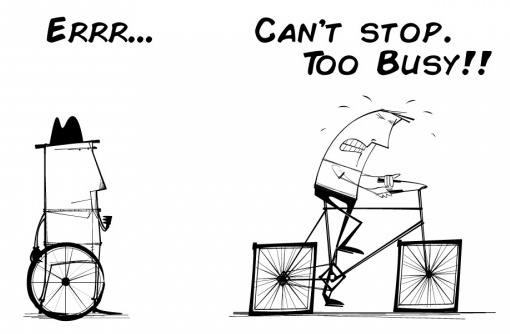
\includegraphics[scale=0.5]{img/toobusytoimprove.jpeg}


\section{State of Art }

As part of the research process has been analyses some aplications
that (although isn't a directly competition) represent the actual
state of art about the kind of sofware we are talking about.


\begin{table}[]
\centering

\begin{tabular}{@{}lllllll@{}}

Feature & classDojo & TeacherKit & A+ & iDoceo & Additio & SMS \\ \midrule

Attendance & \completeValue & \completeValue & \completeValue & \completeValue & \completeValue & \completeValue \\

Discipline & \partialValue & \completeValue & \completeValue & \completeValue & \completeValue & \completeValue \\

Attitude & \partialValue & \completeValue & \completeValue & \completeValue & \completeValue & \completeValue \\

Marks & \noneValue & \completeValue & \completeValue & \completeValue & \completeValue & \completeValue \\

Competencias & \noneValue & \noneValue & \noneValue & \completeValue & \completeValue & \completeValue \\

Rubrics & \noneValue & \noneValue & \noneValue & \completeValue & \completeValue & \completeValue \\

Message & \completeValue & \completeValue & \completeValue & \noneValue & \noneValue &	\completeValue \\

patters & \noneValue & \noneValue & \noneValue & \completeValue & \completeValue & \completeValue \\

reports & \noneValue & \completeValue & \completeValue & \partialValue & \completeValue & \completeValue \\

analysis & \partialValue & \completeValue & \partialValue & \partialValue & \partialValue & \completeValue \\

models and predictions & \noneValue & \noneValue & \noneValue & \noneValue & \noneValue & \completeValue \\

Centralizate and jerarqy & \noneValue & \partialValue & \noneValue & \noneValue & \noneValue & \completeValue \\ \midrule

Total & 58.3\% & 80.5\% & 72.2\% & 	72.2\% & 80.5\% & 99\% \\
\end{tabular}
\caption{Features}
\label{my-label}
\end{table}


\begin{table}[]
\centering

\begin{tabular}{@{}lllllll@{}}

Feature & classDojo & TeacherKit & A+ & iDoceo & Additio & SMS \\ \midrule

Personalization & \noneValue & \noneValue & \noneValue & \noneValue & \noneValue & \noneValue \\

Good UI & \partialValue & \completeValue & \completeValue & \completeValue & \completeValue & \completeValue \\

Buena UX & \partialValue & \completeValue & \completeValue & \completeValue & \completeValue & \completeValue \\

Price & \noneValue & \completeValue & \completeValue & \completeValue & \completeValue & \completeValue \\

Performance & \noneValue & \noneValue & \noneValue	 & \completeValue & \completeValue & \textcolor{ownGreen}{\completeValue} \\

Scalable & \noneValue & \noneValue & \noneValue & \completeValue & \completeValue & \completeValue \\

Data control & \completeValue & \completeValue & \completeValue & \noneValue & \partialValue & \completeValue \\

Multiplatform & \noneValue & \noneValue & \noneValue & \completeValue & \completeValue & \completeValue \\

Centralized & \noneValue & \completeValue & \completeValue & \partialValue & \completeValue & \completeValue \\ \midrule

Total & 44.4\% & 50.0\% & 16.6\% & 	16.6\% & 44.4\% & 99\% \\
\end{tabular}
\caption{Architecture and design}
\label{my-label}
\end{table}

Let's go to start!

%
\chapter{State of Art and first decisions. }

In this chapter, we are going to talk about the state of art in two domains.
On one side we have the analysis of the similar projects or applications that
already exists in the market, which would be the state of art of the problem
that we want to solve and by other side, the technologies that we can choose
to solve this, it would be the state of art to the implementation.

\section{Problem domain}

The developing of a new complete system have no sense if before have not been
analyzed other existent solutions. As part of the research process has been
analyzed some applications that (although is not a direct competition) represent
the actual state of the art about the kind of software we are talking about.
\intro
First, we take a look at the main features that are important in our domain
to see how many applications have covered them. These are a few requirements
analysis but not very formal, we will discuss about this after.
\intro
In the following table, we are going to compare the rest of app with our idyllic
software (with the features we hope it will cover).

\begin{table}[H]
\centering

\begin{tabular}{@{}lllllll@{}}

Feature & classDojo & TeacherKit & A+ & iDoceo & Additio & SMS \\ \midrule
Attendance & \completeValue & \completeValue & \completeValue & \completeValue & \completeValue & \completeValue \\
Discipline & \partialValue & \completeValue & \completeValue & \completeValue & \completeValue & \completeValue \\
Attitude & \partialValue & \completeValue & \completeValue & \completeValue & \completeValue & \completeValue \\
Marks & \noneValue & \completeValue & \completeValue & \completeValue & \completeValue & \completeValue \\
Competencias & \noneValue & \noneValue & \noneValue & \completeValue & \completeValue & \completeValue \\
Rubrics & \noneValue & \noneValue & \noneValue & \completeValue & \completeValue & \completeValue \\
Message & \completeValue & \completeValue & \completeValue & \noneValue & \noneValue &	\completeValue \\
patters & \noneValue & \noneValue & \noneValue & \completeValue & \completeValue & \completeValue \\
reports & \noneValue & \completeValue & \completeValue & \partialValue & \completeValue & \completeValue \\
analysis & \partialValue & \completeValue & \partialValue & \partialValue & \partialValue & \completeValue \\
models and predictions & \noneValue & \noneValue & \noneValue & \noneValue & \noneValue & \completeValue \\
Centralizate and jerarqy & \noneValue & \partialValue & \noneValue & \noneValue & \noneValue & \completeValue \\ \midrule

Total & 58.3\% & 80.5\% & 72.2\% & 	72.2\% & 80.5\% & 99\% \\
\end{tabular}
\caption{Features}
\label{my-label}
\end{table}

\noindent As we can see, there are some apps that are so focused on their specific domain
that is very deficient in the rest. In spite of this are referents in
their area, and their numbers of users are huge (only have been compared apps
that have a good acceptance by users).
\intro
But is not only important the features of the software, because with time and
effort any feature can be added. There are other things in the background that
are really important too and that can be that to grow our app steadily or that crash
when we have thousand of users. We are talking about something as data control,
performance, scalability or centralización (we do not explain in detail each one because
is out of his work but we think is also very important).
And of course, all related to interface and user experience, that in most of
cases can represent the difference between the successful and failure of our
project.
\intro
So, based on it this is our comparative:



\begin{table}[H]
\centering

\begin{tabular}{@{}lllllll@{}}

Feature & classDojo & TeacherKit & A+ & iDoceo & Additio & SMS \\ \midrule
Personalization & \noneValue & \noneValue & \noneValue & \noneValue & \noneValue & \noneValue \\
UI & \partialValue & \completeValue & \completeValue & \completeValue & \completeValue & \completeValue \\
UX & \partialValue & \completeValue & \completeValue & \completeValue & \completeValue & \completeValue \\
Price & \noneValue & \completeValue & \completeValue & \completeValue & \completeValue & \completeValue \\
Performance & \noneValue & \noneValue & \noneValue	 & \completeValue & \completeValue & \textcolor{ownGreen}{\completeValue} \\
Scalability & \noneValue & \noneValue & \noneValue & \completeValue & \completeValue & \completeValue \\
Data control & \completeValue & \completeValue & \completeValue & \noneValue & \partialValue & \completeValue \\
Multiplatform & \noneValue & \noneValue & \noneValue & \completeValue & \completeValue & \completeValue \\
Centralization & \noneValue & \completeValue & \completeValue & \partialValue & \completeValue & \completeValue \\ \midrule

Total & 44.4\% & 50.0\% & 16.6\% & 	16.6\% & 44.4\% & 99\% \\
\end{tabular}
\caption{Architecture and design}
\label{my-label}
\end{table}

\noindent Obviously, only in the hypothetical case of our app is fully developed will cover
all the aspects considered, but before of the research is easy to understand that
is not so difficult cover all with the correct design, architecture or design.
\intro
And we are going to try to give a simple and really little approximation of the way
to achieve that.
\intro
So, \textbf{let's start!}


\section{Implementation domain}


Nowadays we can build almost any kind of software with a lot of differents
language from which to choose, but as if that were not enough there
are also a lot of architectures that are possible to follow, and beside
of this it will be necessary choose where to deploy our software, or how
doc it, or how to manage our work team, etc. A lot of options that it
will be necessary to choose and that can make the difference between the
success or failure of our project. So, what about of these decisions
in this project? We are going to take a look at it, tools, patterns and
\textit{we will take some firsts decisions about it.}

\subsection{Architecture}

Almost any kind software or tool can be built of differents ways, independently
of this behavior or the goals that it must achieve. Some ways are more specific
to achieve some specific behavior and other although useful are not the best option.
Because of this, we need this phase of research, to avoid, as far as possible, make mistakes before to start.

\subsubsection{Kind of software}
We can think of a mobile app, but what happens with desktop users? And even if
we do a mobile app, for what operating system? Too options for to develop a solution
for each one. Based on informal requirements was thought that the best option could be a
\textbf{web app} for a lot of reasons. First of all because is the simplest
way to offer an app that can run on almost any device (with a \textit{
simple\footnote{Actually a browser is one of the more complex pieces of
software, but here is labeled as simple because is a software that the
majority of devices like smartphones, tablet, etc, have by default and for
the most nontechnical people isn't a complex software, nothing could be
further from the truth.}} browser). Also because is the easiest way, with the best
learning curve and to end because can be used a lot of different technologies to the same domain.

\subsubsection{Why microservices?}

When we think about an app, of any type, the most of the time we think of a software
running on a single machine, with more or less hardware available, where all
related to the software are inside of the same machine.
\intro
Now, we hearing all the time about microservices, which are in synthesis the
opposite of the traditional monolithic classical approach in software architecture,
and seem like if your design is not based in this mean you are outdated or your design is directly wrong.
Well, this is not totally true but neither false. The goal of this section is
not describe the advantages and drawbacks of this approach, but yes justify why
is their choice.
\intro
Microservices are actually a variant of SOA\footnote{Service-oriented architecture (SOA)
was first described by Gartner in 1996 and is a style of software design where
services are provided to the other components by application components, through
a communication protocol over a network},that simplify a lot the architecture
of a software system spliting their different systems, doing that work together
to offer the service which the software was design.
Dr. Peter Rodgers introduced the term "Micro-Web-Services" during a presentation
at Cloud Computing Expo in 2005 and as we can see in the following graphic (extracted
using sotagtrends.com) community interest about this emerging technology
has never stopped growing,

\begin{figure}[H]
  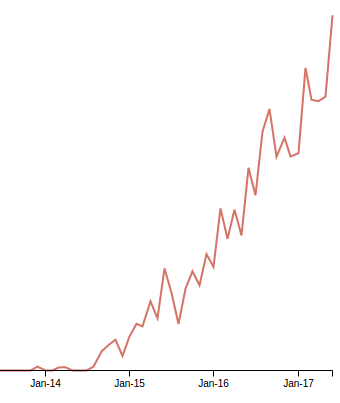
\includegraphics[scale=0.5]{img/graphics/microservices_trend.png}
  \centering
  \caption{Search trend of "microservice" tag in Stack Overflow.}
\end{figure}

\noindent James Lewis\footnote{Principal Consultant at ThoughtWorks and
member of the Technology Advisory Board} and Martin Fowler\footnote{British software developer,
author and international public speaker on software development, specializing in
object-oriented analysis and design, UML, patterns, and agile software development
methodologies, including extreme programming.} are the major defensor of this
arquitecture and these brings us to the canonical definition of microservices:
\bigskip

\begin{minipage}{0.9\linewidth}
        \vspace{5pt}%margen superior de minipage
        {\small
        \textit{"In short, the microservice architectural style is an approach to developing a
        single application as a suite of small services, each running in its own process
        and communicating with lightweight mechanisms, often an HTTP resource API.
        These services are built around business capabilities and independently deployable
        by fully automated deployment machinery. There is a bare minimum of centralised management
        of these services, which may be written in different programming languages and
        use different data storage technologies."}
        }
        \begin{flushright}
            (Lewis/Fowler)
        \end{flushright}
        \vspace{5pt}%margen inferior de la minipage
    \end{minipage}


\noindent Language agnostic, scalable, size ajustables, independently, our system design
splited in litle pieces with this boundaries do this architecture perfect for
our goals, and this is why we take this choice.

\subsubsection{Why polyglot database?}

With mircroservices approach the system will need differents databases to do
some diferent things. In general we can see our
backend like a black box when the data persists in a polyglot database.
That means that the data is saved in differents ways, using different
formats and diferent drivers to manage this. There are a group of
data that would have need be saved with certain relations, due to its nature
and a relational database seem perfect to do this, but this kind of
databases (like MySQL) can be slowly or too heavy for other tasks
of kind of processes, like data analysis.


\subsection{Storage}

With the storage occurs the same, there is a huge list of options to
choose. The fast answer in the most of the cases is: Why do not use a relational
database, as MySQL for example? If we are thinking in a little system
it could be a good choice, always that our data model is adjusted to this kind of system.
But every people knows the deficits and the complexity of the development of a system
with this database. Mainly the performance when we are talking about million
of arrays of objects stored. So, as we was talking before, our goal in this project
is work with a lot of data, of which some are pure relational and another not,
and can be processed by another way, using another engine and database.
\intro
If you have a logical data model like as this project have is not easy choice one
of all database engine to model this. SQL systems is very powerful for some
things but not for another (or not simply) and object oriented databases is
really powerful and simple to develop with it when the data haven't a lot of
relations (although can be modeled also).
so, why choice one between them? Why do not both? This is the approach selected,
build a system with a Polyglot Database, that means: much better select the better
engine for any kind of data instead of trying to use the same for all.
\intro
And this approach joined with microservices architecture give us the first
Conceptual design of our system, where each microservice have their domain work and their
own data, using for their own database engine, and
Until their own language is it will be required.
\intro
So, focused on this project, we are going to use mainly two systems, SQL
relational database system in a service (we will talk more about it after),
and a NoSQL service, in this case, Google Datastore, a fast and lightweight
engine to mange an object oriented database.
\intro
At the moment of to write this chapter had been evaluated MongoDB as the best
choice, but the facilities of the platform selected (detailed after) was made
that the G. Datastore was selected finally. Beside of this if the project are
rebuild now have not doubt, Mongo will be selected after the experience ( the
reasons will be explained in more detail in the conclusion of the work).

\subsection{Code strategy}

Entire project will be stored in a single repository, using git as control
versions system.

\subsubsection{Version Control System}

Git\footnote{Git is a free and open source, distributed version control system
created by Linus Torvalds} is the perfect tool to achieve maintain a more o
less easy workflow between developers minimizing the risks, and the huge list of
plugins to different software and IDEs do this perfect to work, dismissing another
as Subversion, Mercurial, Fossil, or Bazzar.
\intro
The reason to use a single repository is that the mechanism to maintain the
consistency between projects is not easily enough to do the develop agile.
In spite of, git offers us a lot of tools that can improve enormously our
workflow, as the Git Submodules\footnote{Submodules allow you to keep a
Git repository as a subdirectory of another Git repository.
This lets you clone another repository into your project and keep your commits
separate.}, or Git Hooks\footnote{Git has a way to fire off custom scripts when
certain important actions occur. There are two groups of these hooks:
client-side and server-side. Client-side hooks are triggered by operations such
as committing and merging, while server-side hooks run on network operations
such as receiving pushed commits} between another.

\subsubsection{Hub}

For another hand we have to do another choice, select the remote hub of our repositories
or Git repository hosting service. The most popular for some years has been GitHub,
are a web-based Git or version control repository and Internet hosting service.
It offers all of the distributed version control and source code management (SCM)
the functionality of Git as well as adding its own features,
launched at 2008
but there are other options as Bitbucket\footnote{web-based hosting service
that is owned by Atlassian, used for source code and development projects that
use either Mercurial (since launch) or Git
launched at 2008},
SourceForge\footnote{another system launched at 1999} and especially
GitLab\footnote{launched at 2011, was written by Dmitriy Zaporozhets and Valery
Sizov from Ukraine. The code is written in Ruby. Later, some parts have been
rewritten in Go.} (with a big grow ultimately).


\subsubsection{Develop workflow}

Another of the main problem easy to find in the develop when are involved
few people is the organization of the contribution of a repo, but if the project
is composed of few subprojects, this can be worst. For this reason was choose the
strategy to have an only repo with subfolders.
So, took this decision remains to be defined how will work the repo in the
different phases or the develop.
\intro
To do this, we will follow the standard, using branches to develop features and
maintain a good state of the versioning of project.
\intro
So, as we can see in the picture, we are going to use \textit{develop} branch
to do the develop, where we are going to work in minimal changes and will do
a fork when we want to do some representative change in the code, as new functionality or
some big correction.


\begin{figure}[H]
  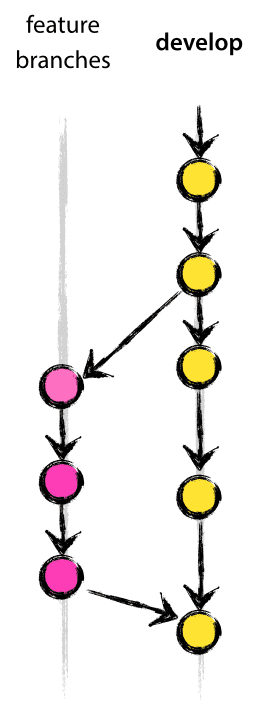
\includegraphics[scale=0.25]{img/git/feature_branches.png}
  \centering
  \caption{Workflow with features branches}
\end{figure}

\noindent For other hand when the all code to launch a final release we will fork the
repo in a \textit{release} branch to while the team continue with the develop
in the mainly develop branch ot in a issue form of this another part of the
team (or itself, is the same), will prepare the code to production, taking a look
because there are some bug, fix it and when all are testend an correctly working
put the project in exactly this verison in master (doing a merte) and this is
when officially a new version of program will be launched.

\begin{figure}[H]
  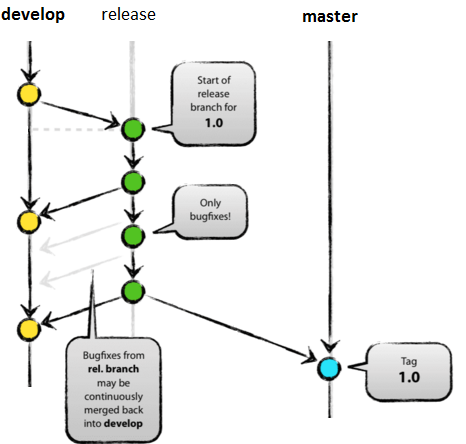
\includegraphics[scale=0.5]{img/git/release_branches.png}
  \centering
  \caption{Workflow with releases branches.}
\end{figure}

\noindent There are some variations of this standard workflow but for this kind of project
is perfect.

\subsection{Languages and frameworks}

As has been said before, almost any kind of software can be builded at infinite
ways, and this start with what language can do this. This means it could be
builded with Java, Ptyhon, C++, Go, Ruby, JavaScript, PHP,  (only talking about
backend) and with another list to frontend, in this deep list of possibilities,
we choose the most flexible and powerfull of all of them, Python and JavaScript.
\intro
Python because is one of the most simplest and powerfull languages nowadays, and
JavaScript because is all an standard in the industry. Obviously the choise is
based also in the fact of both languages are really supported of community, have a
good learning curve and a lot of projects and systems are based in them.
\intro
JavaScript has been selected becuase Angular is writte in it. AngularJS is the
most powerfull framework nowdays to buil fas, clean and powerfull web apps.
\intro
To exchange data between service we need to select a idiom which the services
will talk, which them will exhange information. That's mean mainly select how
will transform the objects anda data structures that servicres manage to be able
sender across the net.
\intro
We have some data serialization solutions, some very popular and another most
specific of very focused domains. So, the most commons are Json, Yaml,
Bson and ultimately MessagePack. Each have their owns benefits and drawbacks but
the selection has been easy, JSON.
\intro
\textbf{XML}
\intro
Extensible Markup Language, is a markup language, defined v1.0 by
W3C\footnote{World Wide Web Consortium, founder by Tim Berners-Lee at 1994 at MIT
(Massachusetts Institute of Technology) the consortium is made up of member
organizations which maintain full-time staff for the purpose of working together
in the development of standards for the World Wide Web.} This is an example:

\begin{lstlisting}[language=xml,frame=none,numbers=none]
  <exam>
    <result>5.8</result>
    <type>Partial</type>
    <subject>Science</subject>
    <date>17-06-2018</date>
  </exam>
\end{lstlisting}


\noindent \textbf{JSON}
\intro
JavaScript Object Notation, is an open-standard file format that uses
human-readable text to transmit data objects consisting of attribute–value pairs
Douglas Crockford originally specified the JSON format in the early 2000s;
two competing standards, RFC\footnote{ Request for Comments, is a type of
publication from the Internet Engineering Task Force (IETF) and the Internet
Society (ISOC), the principal technical development and standards-setting bodies
for the Internet. were invented by Steve Crocker in 1969 to help record
unofficial notes on the development of ARPANET} 7159 and ECMA\footnote{Ecma is a
standards organization for information and communication systems founded in 1961
to standardize computer systems in Europe.}-404, defined it in 2013.
The ECMA standard describes only the allowed syntax, whereas the RFC covers some
 security and interoperability considerations.
\intro
In spite of A restricted profile of JSON, known as I-JSON (short for "Internet JSON"),
defined in RFC 7493, is not as popular as original. This is an example:

\begin{lstlisting}[frame=none,numbers=none]
  {
    "title": "The Picture of Dorian Gray",
    "author": "Oscar Wilde",
    "date": "July 1890"
  }
\end{lstlisting}


\noindent \textbf{YAML}
\intro
Yet Another Markup Language is commonly used for configuration files, but could
be used in transmision also, YAML 1.2 is a superset of JSON, whitch Latest release1.2
(Third Edition) was published at (1 October 2009; 7 years ago), YAML was first
proposed by Clark Evans in 2001.

\begin{lstlisting}[frame=none,numbers=none]
  ---
  invoice: 34843
  date   : 2001-01-23
\end{lstlisting}


\noindent \textbf{BSON}
\intro
Binary JSON, is a computer data interchange format used mainly as a data storage
and network transfer format in the MongoDB database.
MongoDB represents JSON documents in binary-encoded format called BSON behind
the scenes. BSON extends the JSON model to provide additional data types,
ordered fields, and to be efficient for encoding and decoding within different languages.
\intro
\noindent \textbf{MessagePack}
\intro
Byte array is an efficient binary serialization format, like JSON but faster and smaller.

\begin{lstlisting}[frame=none,numbers=none]
{"compact": true, "schema": 0}
27Bytes

82 A7 compact C3 A6 schema 00
18bytes
\end{lstlisting}
\noindent And another aprox as zerorp, It builds on top of ZeroMQ and MessagePack

\subsubsection{Protocol}

Microservices must talk and can do this by differents ways. So, we are going to
take a look over more interesting for us.
\intro
The first that we are talking about is \textbf{REST}. Representational state transfer or
RESTful Web services are one way of providing interoperability between computer systems on the Internet. REST-compliant
Web services allow requesting systems to access and manipulate textual representations
of Web resources using a uniform and predefined set of stateless operations. Other
forms of Web service exist, which expose their own arbitrary sets of operations such as
WSDL and SOAP
\intro
On other hand we have \textbf{RPC}. In distributed computing, a remote procedure call  is when a computer program
causes a procedure (subroutine) to execute in another address space (commonly on
çanother computer on a shared network), which is coded as if it were a normal (local)
procedure call, without the programmer explicitly coding the details for the remote interaction.
\intro
And finally \textbf{gRPC} . It is an open source remote procedure call (RPC) system initially developed at
Google. It uses HTTP/2 for transport, Protocol Buffers as the interface description
language, and provides features such as authentication, bidirectional streaming and
flow control, blocking or nonblocking bindings, and cancellation and timeouts.
It generates cross-platform client and server bindings for many languages.
We will talk a bit more about this in the Develop chapter.


\subsubsection{Testing}

The tool that we will use for any testing involved in the backend of the project
will be PyTest. Launched at 2004 by Holger Krenel is one of the most complete
suites for testing over Python.
Is really easy to use and allow do some things that is very difficult with another
frameworks as built-in \textit{unittest} python package, somethings as the use of
fixtures of or the amount of plugint that it has.
\intro
Focused on the problem it will be used to make all unittest of the core of services,
libraries and auxiliary programs and testing the entire functionality of the service
when it has a role of black box.


\subsubsection{Documentation}

As is saided the tool Sphinx is used to build the doc of the service.
That basically inspect the code files mixing this with all the files
that we write (pure doc) to show this as a web based documetnation
(easy to read and understand).


\subsection{Platforms}

Today, with the explosion of the cloud is needed a lot of infrastructure that support
all that all companies that want to migrate thier bunisses model to cloud need. the possiblite
come from of the companies that offer solutions to do this, and another that after
was introduced in the same bunisses.
So, actually there are a lot of companies that offer some solutions to sofware (not necessary)
companies to work with cloud to build their solutions and cloud computing easily.
\intro
There are a lot but only few are the big in this busineess. And alwyas respond to some
model IaaS (Infrastructure as a Service)
AWS, G Computer Engine, Rackspace Cloud, vCloud PaaS (Platform as a Service)
Google App Engine, Heroku, SaaS (Sofware as a Service) Google Docs, Salesforce, Dropbox, Gmail
\intro
\textbf{Amazon Web Services}
\intro
Launched at 2006 The most popular include Amazon Elastic
Compute Cloud (EC2) and Amazon Simple Storage Service (S3)
\intro
\textbf{Microsoft Azure}
\intro
is a cloud computing service created by Microsoft for building, testing, deploying,
and managing applications and services through a global network of Microsoft-managed
data centers. It provides software as a service (SAAS), platform as a service and
infrastructure as a service and supports many different programming languages,
tools and frameworks, including both Microsoft-specific and third-party software and systems.
Azure was announced in October 2008 and released on February 1, 2010 as Windows
 Azure, before being renamed to Microsoft Azure on March 25, 2014.
\intro
\textbf{IBM BlueMix}
\intro
is another platform.
\intro
\textbf{Heroku}
\intro
Is a cloud platform as a service (PaaS), founded by James Lindenbaum in 2007 at
 San Francisco, California, supporting several programming languages that is used
 as a web application deployment model.
 Heroku is said to be a polyglot platform as it lets the developer build,
 run and scale applications in a similar manner across all the languages.
 Heroku was acquired by Salesforce.com in 2010 for 212 million of dollards.
\intro
\textbf{CloudFoundry}
\intro Is an open source, multi cloud application platform as a service
(PaaS) governed by the Cloud Foundry Foundation, a 501(c)(6) organization.
The software was originally developed by VMware and then transferred to Pivotal Software,
a joint venture by EMC, VMware and General Electric launched at 2011
\intro
\textbf{Google Cloud Platform}
\intro Is a suite of cloud computing services
that runs on the same infrastructure that Google uses internally for its end-user
products, such as Google Search and YouTube.Alongside a set of management tools,
it provides, a series of modular cloud services including computing, data storage,
data analytics and machine learning.
\intro
And is this which was selected.

\subsection{Documentation}

To do the documentation of the code as in the rest of sections, we have a few options
to choose. So, as the backend is fully developed in Python we are going to use some python
especially documentation framework and in this case Sphinx\footnote{Sphinx is a
simple and powerful Python-based documentation generator.} has been selected.
\intro
For another hand, to the front, especially talking about Javascript with AngularJS
we do not have the need to a doc because the docstrings have been sufficient,
and neither have been found any really good tool as Sphinx for them.

\subsection{License}

In this project, we are going to use GNU General Public License v3 (GPL-3)
to license our code.
There are a lot of licenses available, but it meets all our needs,
this is a little summary of this:

\begin{table}[H]
  \centering
  \begin{tabular}{ l | c | r }
    Can &  Cannot & Must \\
    \hline
    Commercial use    & Sublicense    &  Include original \\
    Modify            & Hold liable   &  State changes \\
    Distribute        &               &  Disclose source \\
    Place warranty    &               &  Include License \\
    Use patent claims &               &  Include Copyright \\
                      &               &  Include Install Instruction \\
  \end{tabular}
  \caption{License characteristics summary.}
\end{table}

%
\chapter{Requirements}

In this chapter, we are going to describe which are the requirement that our system has.
It will be used User Stories\footnote{A user story is an informal, natural language
description of some features of a software system. See bibliography to know more.}
methodology which it will be talked a bit more in the next chapter.
This tool will be useful to identify the requirements of the system by a
human readable way., removing all possible layer between design and traditional
requisites specification process.
\intro
User stories can be very minimal (unit) and very general. That mean that we
can do a user story that is a simple requirement or a very general issue.
If the criteria to follow is to do very minimal users stories, we could be
hundred of them, so in this case, is better have an upper abstraction level
to have fewer user stories but with more content, at least when is the
first time that the team uses this methodology.

\section{Minimal user requirements}

The managers of the center can't have a precise idea about which must be the
functions of the software. They have a clear idea about what kind of process in
their daily work there are the heaviest and consume more paper, that is which
they want to digitize, but they have not thought about navbars, icons, colors palettes,
user interfaces design or something like this.  They have abstract ideas that will
need dimensioning and shaping but which in synthesis offer the minimum system requirements.

\subsection{General needs}

these are the general requisites that customers have, independently of the logic of the application.
We are talking about software and it will need run in somewhere and must be cheap
and easy to run.
At first, there are not any pre-requirements. Maybe they prefer it can run in
devices like smartphones, tablets, laptops,
but they do not have a good technical knowledge and for they are indifferent that
it will be a native app, a web app or some strange artifact.
\intro
On the other hand, exists an essential requirement, must be run on any device for
the same person, independently of the machine where it be (sometimes in laptop
and others in a smartphone, for example).
\\
See user stories related: GN-1 to GN-3 on appendix A.


\subsection{Academic Management System}

As we can imagine, a center have a lot of differents kind of relationships,
and as an obligatory part of the system, it must be offered a simple way to manage this.
Teachers impart subjects to a group of students (called classes), students are
enrolled in subjects, and so on.
\\
See user stories related: AMS-1 to AMS-7 on appendix A.

\subsubsection{Attendance Controls}

This is one of most important process to digitize, the amount of data that is saved on
paper make impossible to manage fluently and much less  analyzing them.
They need a simple way, a simple interface to do this that allow they to save time
(doing it, analysis and management it), paper and effort.
\\
See user stories related: AC-1 on appendix A.

\subsection{Class Controls}

A part of manage of classrooms they must offers a say to follow the students
evolution in class, behavior, positives and negatives and another lot of things
like paper save, time and effort as section above.
\\
See user stories related: CC-1 on appendix A.

\subsection{Marks}

As another process that more paper consumes is the marks management.
They want a system that simplify the process of insertion, analysis, and management.
Without any special idea in mind are open to any good user interface that simplifies it.
\\
See user stories related: MRKS-1 on appendix A.

\subsection{Disciplinary Notes}
It also must provide a management of this kind of notes, in which a bad behavior
of a student is saved, managed and fully reported to the specific users inside of
app, as tutors, pedagogue, etc, for example.
\\
See user stories related: DN-1 to DN-2 on appendix A.

\subsection{Simple and advance reports}

Another part interesting for they is to improve the reports that they obtain from
their data. The on paper support do this almost impossible to big scale, an
important feature must be do this possible. Advanced reports about a lot of kind
of items, like students, the state of subjects, marks, etc, in seconds with some clicks.
This will improve the take of decisions and will do better meetings with better
decisions based on good and contrastable data.
\\
See user stories related: SAR-1 on appendix A.

\subsection{Autonomic Official System Connection}

The national system of education in which this center is framed have differents
informatic regional systems. In this case, in Andalucia, where the center is, it called
\textit{SENECA} (other in other places of the country). All public and semipublic educational
centers need save data in this systems necessarily, and this haven't a simple public
API where connect us. They must be done dirty way, making a mixed mode way to simplify
the download and download of data that minify the interaction with the official system.
\\
See user stories related: SNC-1 on appendix A.

\section{Minimal system requirements}

The system, as if it was another user has their own requisites,
and can be handled as normal user stories.
So, with the architecture that we are talking about all parts of the system
(the microservices) must be independent and low coupled also must be able to run
in different places using always the same communication protocol (API Rest in this case).
These are not a lot of requisites but are indispensable to the system has the properties
that we expected.
\\
See user stories related: MSR-1 and MSR-2 on appendix A.

%
\chapter{Planning}
\section{Methodology and planing.}

In this project, we are going to use an agile methodology.
This kind of methodologies looking for alternatives to traditional project management.
Agile approaches help teams respond to the unpredictability of changes.
Not only the team has been ready to some change, it knows that they will happen.
\intro
Exists a lot of variants of the same philosophy, Lean Software, Kanban,
Extreme Programing or Scrum, between others.
All follow the same goals but they do with differents ways.
\intro
We are going to use Scrum (\cite{scrumbook}) because some members of the team had some of experience
in it and is the most used in the world of the agile approach.
Is not the goal of this work explain in detail all characteristics of the system,
but we are going to comment the most important to understand the planning.
\intro
We are going to split the six months approximately of time in two weeks slices.
Each slice will be a sprint , a piece of time where will work a very bounded part
of the project, based on very specified issues, with some special characteristics.
All these issues are based on some user story (maybe not directly).
\intro
In SCRUM, almost everything is related with these sprints. So, we have the most
important parts, as the Sprint Planning, Daily Scrum, Backlog and the Sprint
Review Meeting. With these elements, we have enough to start to develop.
The process to follow is very easy. In this case is a bit contradictory because
SCRUM does not understand of deadlines, only of \textit{Minimun Product Value}
and here we follow a planning, but will work anyway.
\intro
So, to start we need split the high priority user stories in real issues (as a
GitHub issues for example), little problems to solve some concrete problem,
labeling this with the priority of the user history.
After we do this, we need to estimate the complexity of this issues, using some
tool as Scrum-poker-cards (see redbooth github repo) and app.  When we have this
we need put in the sprint (2 weeks of work) all issues that we think that we can
to complete, and this will be our sprint.
\intro
There are a lot of details that we are missing out but is not important to explain
the essence of the system.
So. the issues that for any reason will not put in the next sprint will be put
in the backlog (a queue of tasks) where will be recovered from next.
The role of the estimation is very important because do that the team know each
other and knows how many lines of code can produce the whole team (independently
where we are woking at this time).
\intro
So, to give a general image of all project development we are going to split all
issues (coarse-grained) to can to see where would put each issue in general calendar.
Thus we can to know if we are at time in our long-term planning (independently or
our sprint, the dev team and the sales team work with differents concepts of time)
and will be (more or less) easy try to correct or analyze retrospectively.
\intro
This having this said this would be our Burndown chart, that beans, the normal
evolution of remained work to obtain a release with the conditions and deadline
putting ourself.

\begin{figure}[H]
  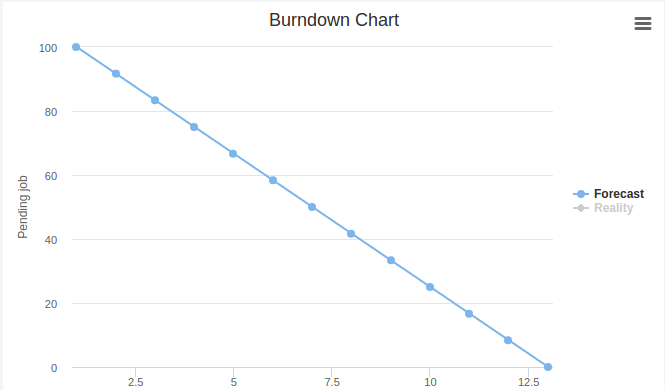
\includegraphics[scale=0.4]{img/graphics/burndown.png}
  \centering
  \caption{Burdown estimation chart.}
\end{figure}

\noindent Now is where play the mechanism Sprint Planning, Daily Scrum and the Sprint
Review Meeting. For each sprint of this thirteen, we must do a sprint planning
to know what issues are inside and which would put in the backlog and another
meeting to review the evolution of sprint.Normally another meeting must be done
diary, but in this case with the form of the team is not possible, so instead of is important, is not at the rest.

%
\chapter{Design}

Once the requirements have been decided, is time to make the design of the system
 that will do all needed to cover them. First we are going to take a look over
 the general arquitecture, the distribution of the domain of the services and
 how delimit their behaviour and communications with each others to after enter
 each one to know how work in each domain and how have been solved all problems
 that this design present.

\section{Responsabilites distribution}

At the moment that we decided split the functionality of the system between
services we found the problem that how decide which is the domain

At the moment that we decided split the functionality of the system between
services, we found the problem that how decide which is the domain of each one.
In the majority of the cases we are begining from a monolithic system that we
want split, in this case is some like this but at first it was thinked to be splited.

In the common app (whatever kind of it) we have three well defined layers, user
interface, logic and storage, something as common MVC\footnote{Model–view–controller
(MVC) is a software architectural pattern for implementing user interfaces on
computers. It divides a given application into three interconnected parts in
order to separate internal representations of information from the ways that
information is presented to and accepted from the user, user interfaces pattern,
introduced by Trygve Reenskaug into Smalltalk-76 at Palo Alto Research Center in the 1970s}
A part of user interface make the necessary to present the info and offer the
way to interact with this to the user while the logic layer do this possible
doing the logic steps to work with data structures saved in some kind of storage.

There are some frameworks as Django wherein all this layer can be developed
toguether, is not strange their popularity, but if we use other as AngularJS
this only help us in the user interface layer, not in the rest, but for other
hands have another advantages.

So, that as it may, this would be the more simple schema to start to work in
our domain, with the difference that we work with service instead of layer in a
single program, but essentially, the concept is the same.

As we can see in the next picture, we will have a user interface, when  will
builded all views and controllers that work with this to buil complete user
interface, a logic section layer, here labeled as APIGmService (as a first
approach) that will do the logic of the system, transform the data,
restructuring and offering the interaction form UI to database.
And at end, the database system, mainly a engine of the database and the drivers
neccesary to work with the.

\begin{center}
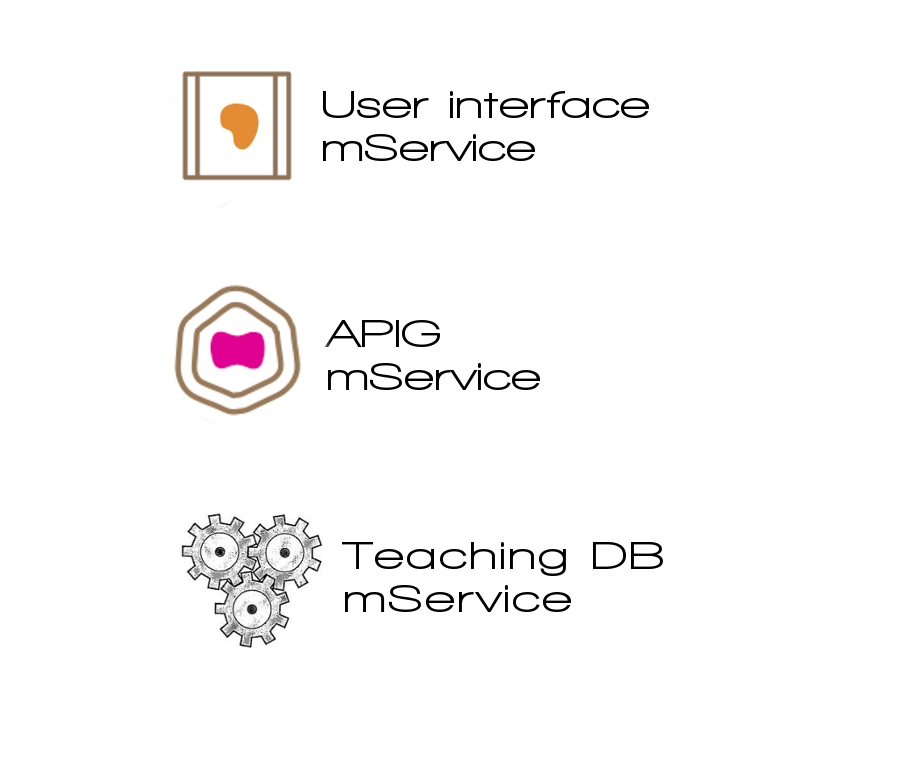
\includegraphics[scale=0.3]{img/graphics/initial_microservices_distribution.png}
\end{center}

As we can imagine this work fine, is compact and stable when we are talking about
the same code in the same machine but now we are going to split that in
different services, maybe runing at diferents places and maybe in different
languages, so when we talk about split the domain is about split the logic with
the database access layer.

Next picture show us perfectly what are talking about. This is an example
of migration from monolithic to microservices from Nginx resources.

\begin{center}
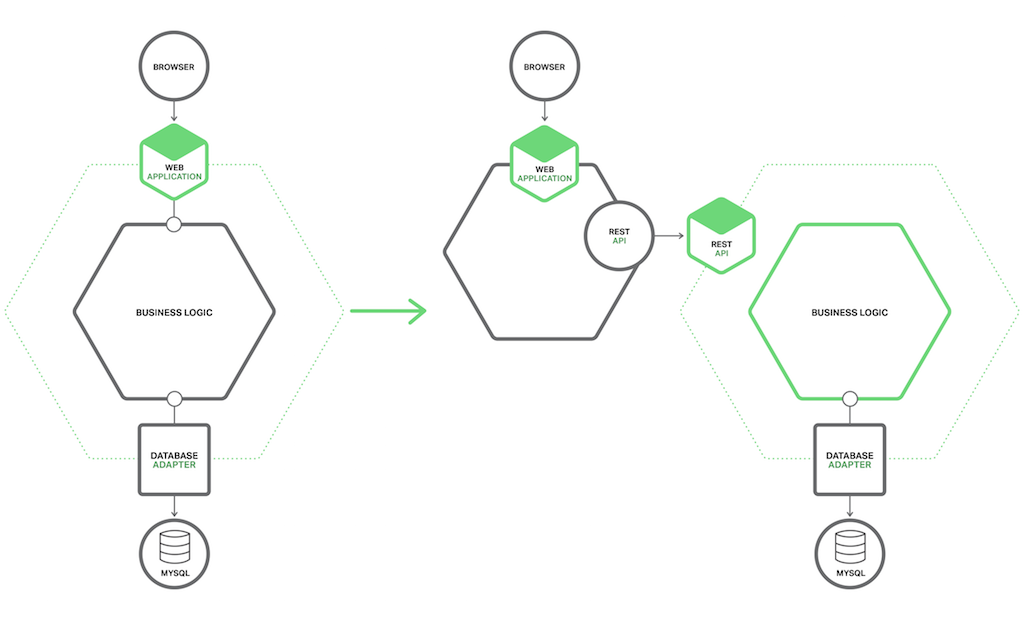
\includegraphics[scale=0.4]{img/graphics/refactoring.png}
\end{center}

So, for us, each service will be always mainly the same components,
communication protocol and logic layer. Database layer is always optional,
a service can be do some logic without need a database, imagine a simple service
to do calcs, that consume the data from another service or act as third party
services gateway, a social network, a payment service, whatever.

Coming back again to our problem we have decided to split all the back end in
four services that will cover the domain of the problem, following a Domain
Driven Development principles. Each one will be described with details after,
for now, only a some reasons that why is so. We need a logic part that control
any call to the system, some as gateway that act as dispatcher of request, that
call to the service (maybe not only one) that can help it to resolve the requests
and give back the info. For another and, we need cover all requierements specified,
and to achieve this we  are going to design three services that split all logic
issues, teaching database, students control and analysis microservice. All toguether
compose the backend of the app.

\begin{center}

\includegraphics[scale=0.3]{img/graphics/backend.png}
\end{center}

Further on we will talking about the reason to choose API Gateway as pattern.


Diferents aproximations in the two mainly platforms to work:

\begin{center}
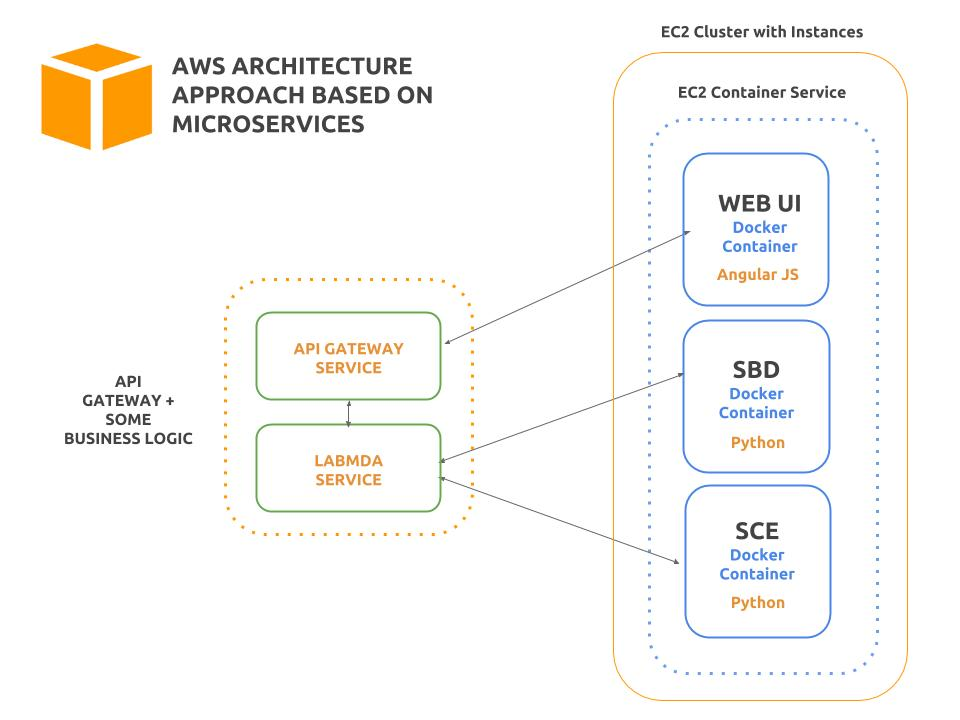
\includegraphics[scale=0.35]{img/graphics/aws_approach.jpg}
\end{center}


\begin{center}
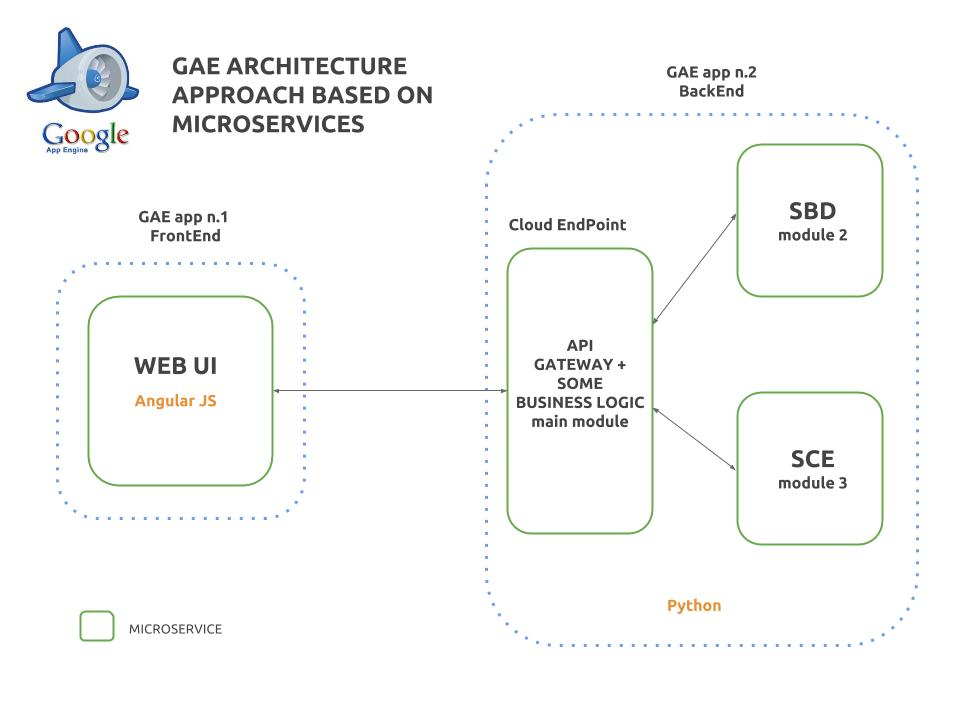
\includegraphics[scale=0.35]{img/graphics/gae_approach.jpg}
\end{center}



This is the complete snap of the system in their final distribution of the
fuctionality between the services.

\begin{center}
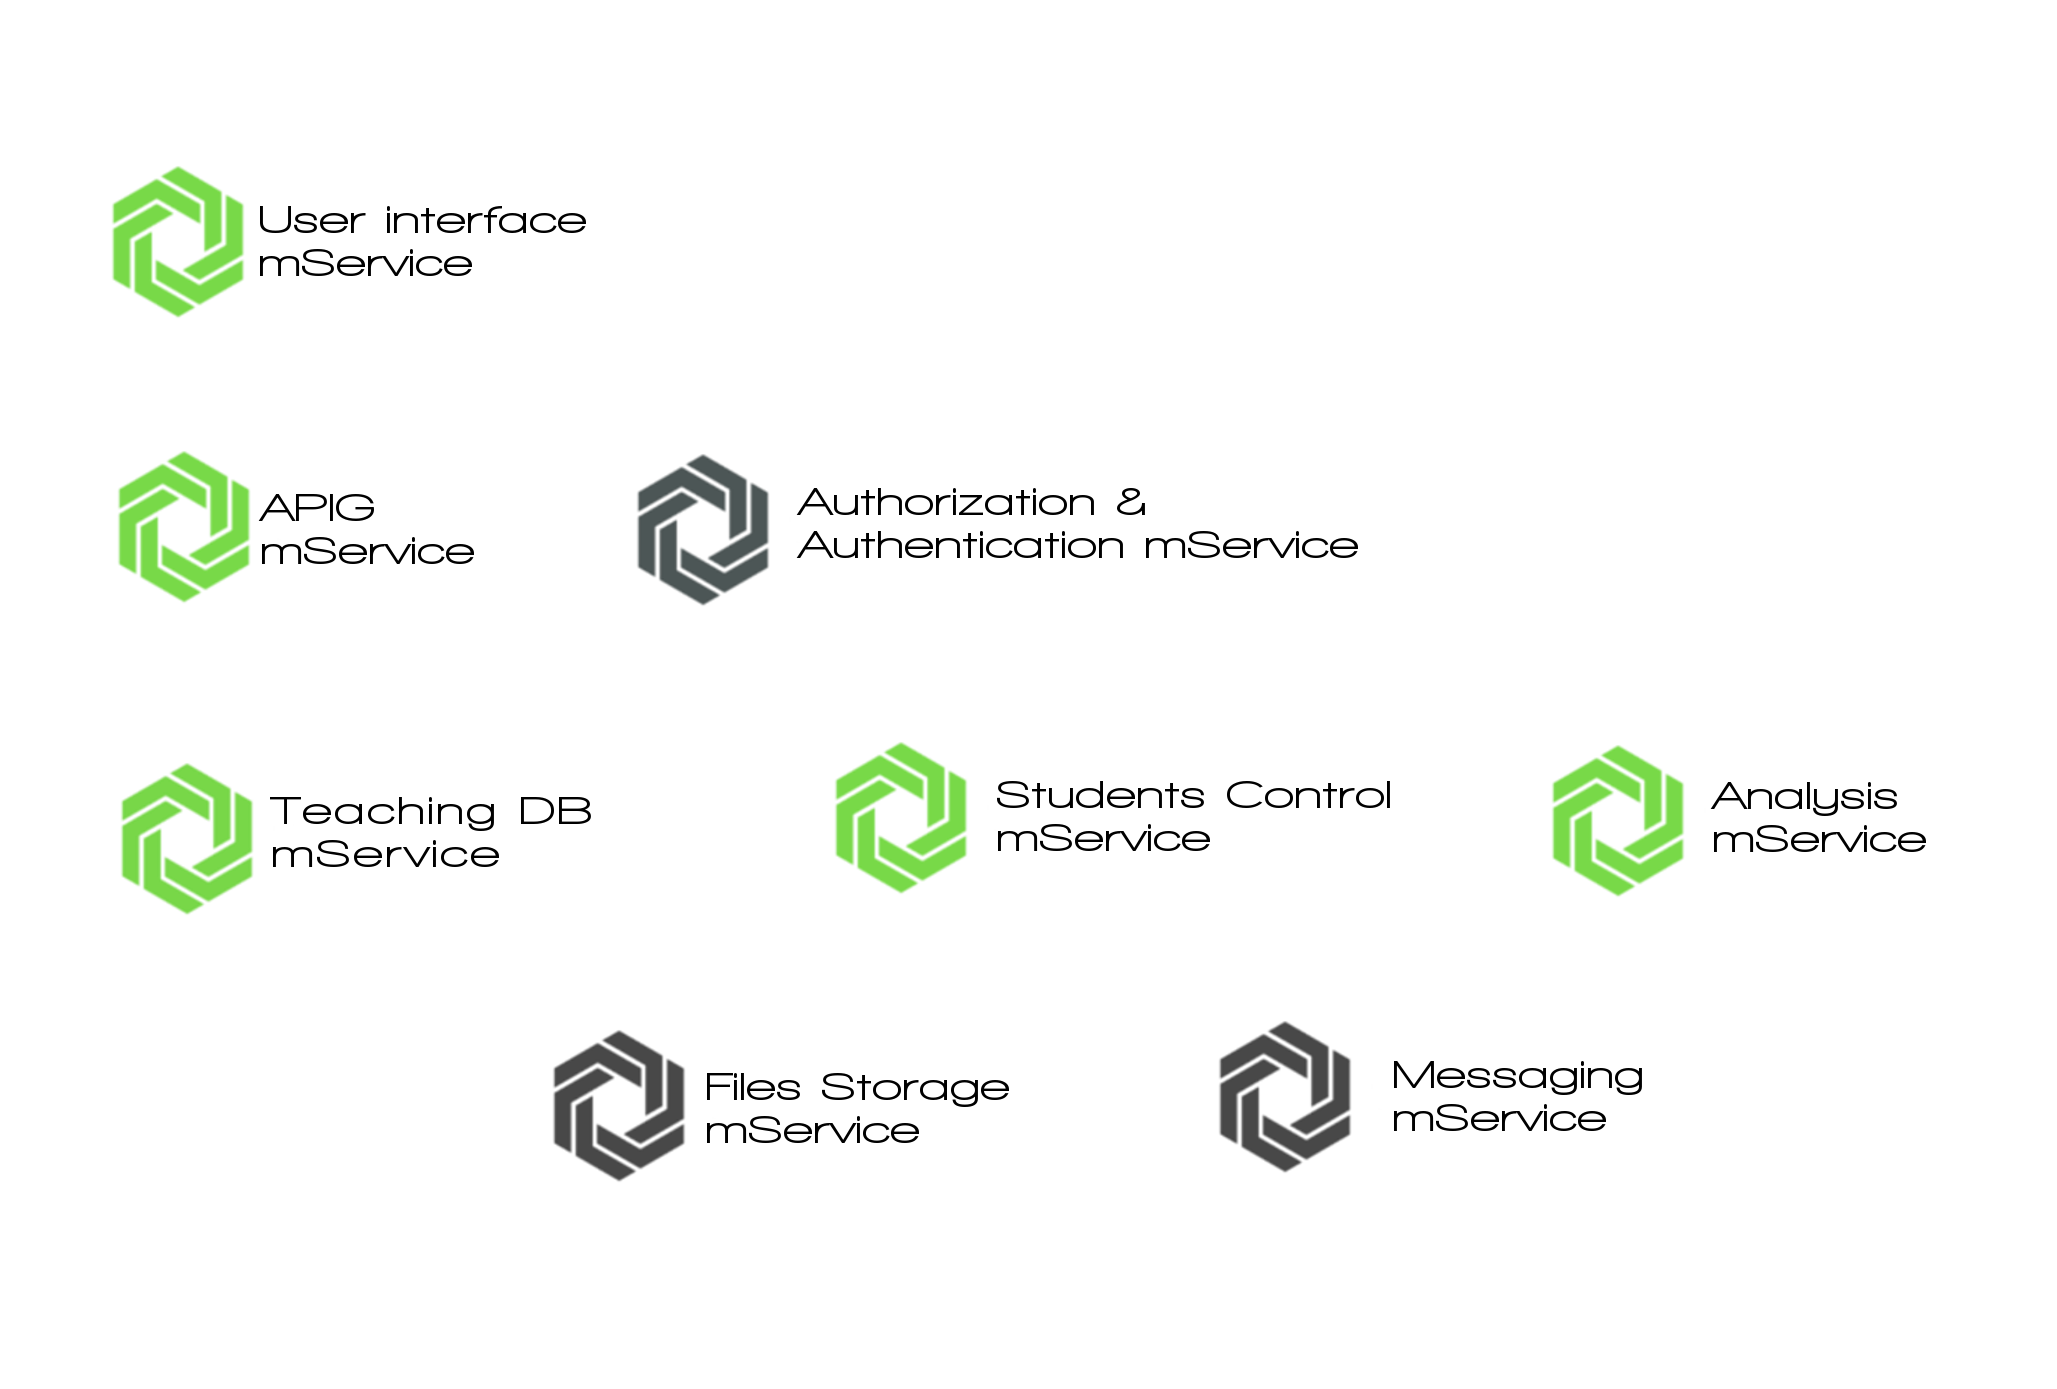
\includegraphics[scale=0.22]{img/graphics/final_microservices_distribution.png}
\end{center}

This is the real situation of the develop

\begin{center}
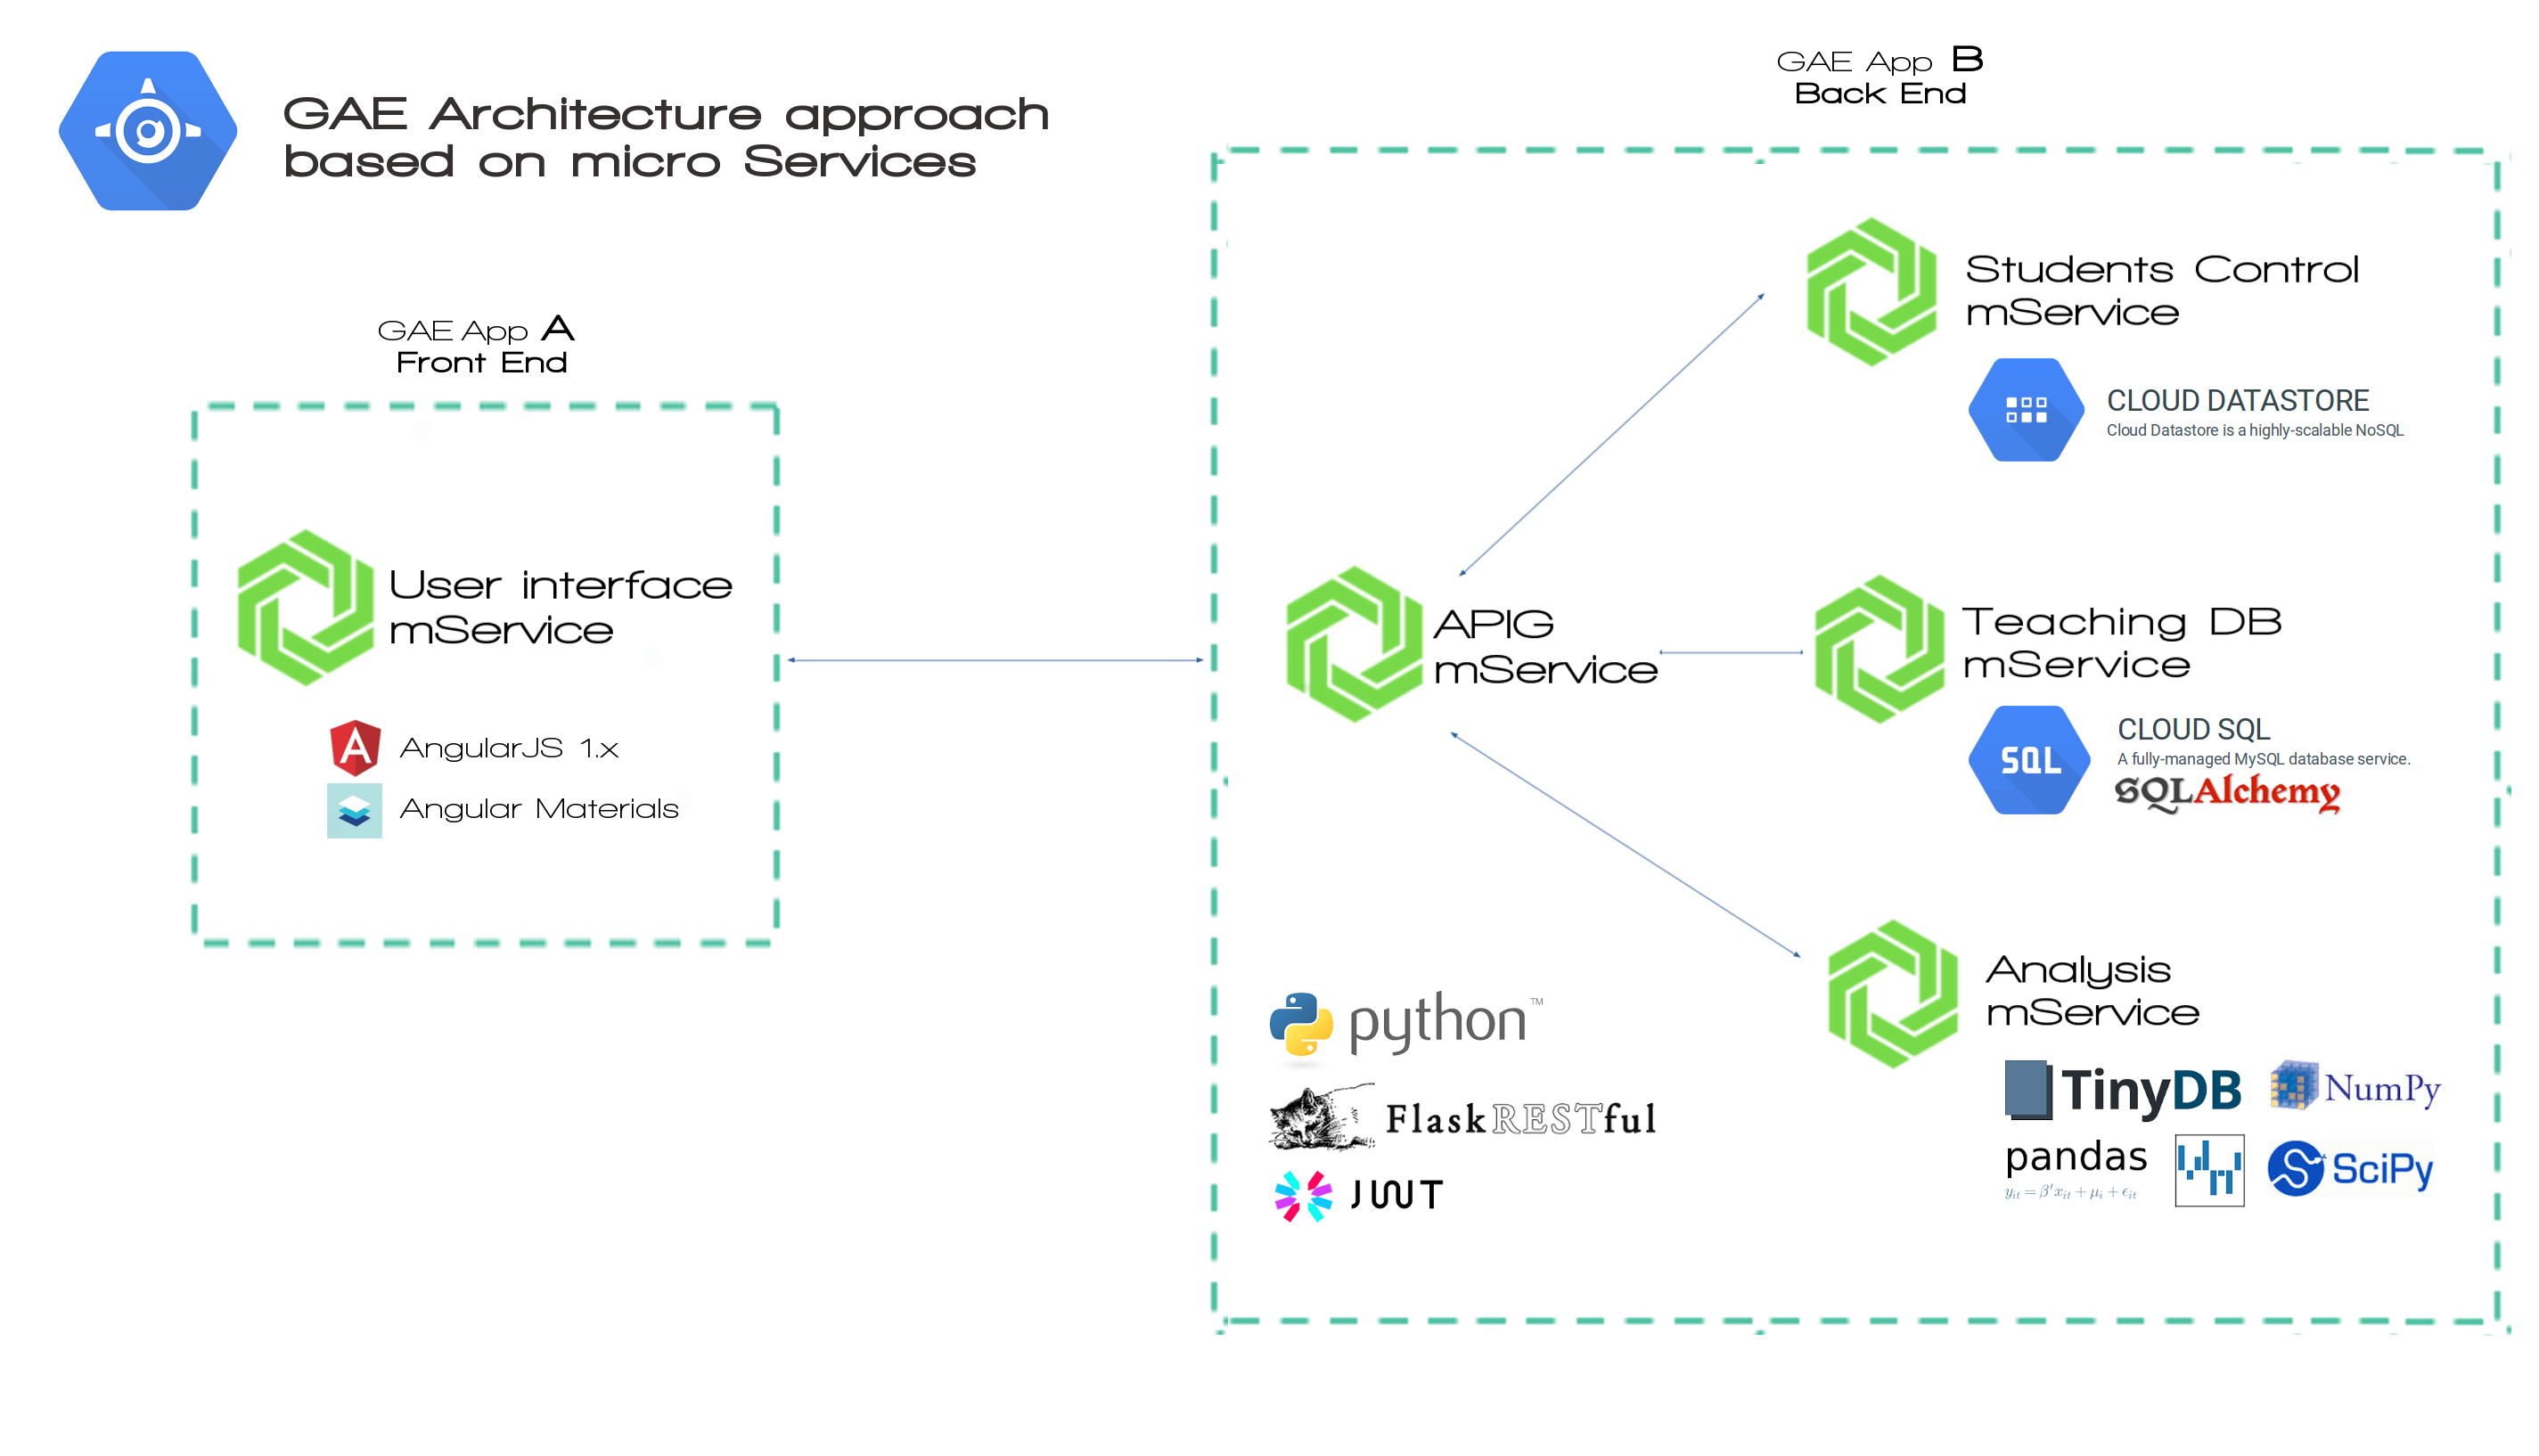
\includegraphics[scale=0.15]{img/graphics/GAE_final_architecture.png}
\end{center}

\subsection{API standar status code cases}

CODIGOS Y POR QUE ELEGIMOS LOS QUE ELEGIMOS

\subsection{Pesistence Strategy}

  Metadata parameters
  createdBy       INT,
  createdAt       DATETIME,
  modifiedBy      INT,
  modifiedAt      DATETIME,
  deletedBy       INT,
  deletedAt       DATETIME,
  deleted         BOOL,

\section{API Gateway microService}

On the other had with docs something similar happens, don't have sense
write a doc defining the behaviour of all sections of api gateway
if this doc already exists in each service. It's redundant and complex
to mantain. Because of this a simple approach is link the docs to
services docs, so the task of write it relegate to them.


\begin{center}
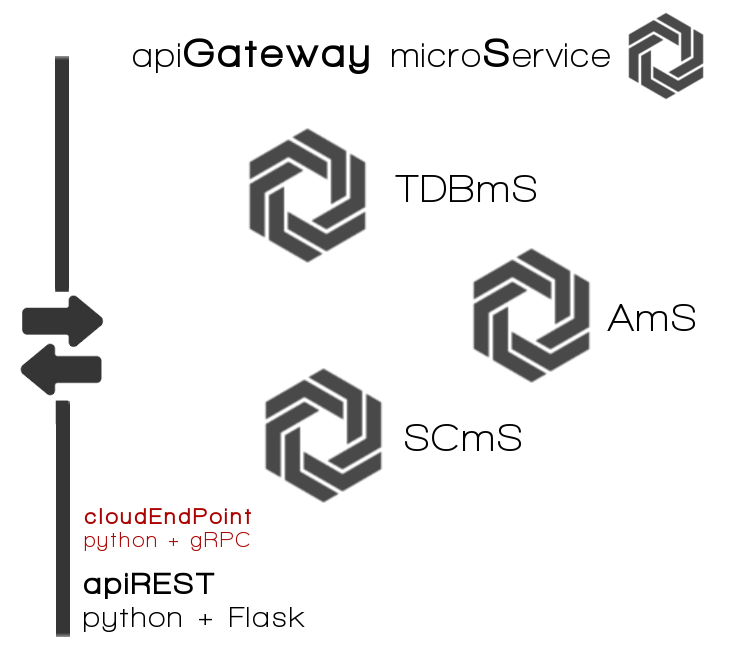
\includegraphics[scale=0.35]{img/graphics/apigateway.png}
\end{center}

\subsubsection {API Definition}






\subsection{Teaching Data Base microService}


This mService offers the managment of the teaching of the center.
This means that persist in a relational database all relations between
teachers, students, subjects, etc, and all resource availables to
make this posible throuhg an api.\bigskip

This like the rest offers his resource throuhg an api writed in Flask
(follow the same architecture that all).

The engine to save all these relations is MySQL, for many reasons,
mainly because is the best known engine and in which it has some experience
and also because GCP offers as a cloud product Google Cloud SQL Databases.
Until recently only offerts MySQL but now (since March of 2017) they
offer also PostgreSQL.

\subsubsection{Design}






\subsubsection{Access Library}

In the old version it was a little ORM that offers simple methods
to access data transform this in SQL raw sencentes. Now this library
is only a wraper of the SQLAlchemy to keep apart the apirest of the
service to the database access layer.

\begin{center}
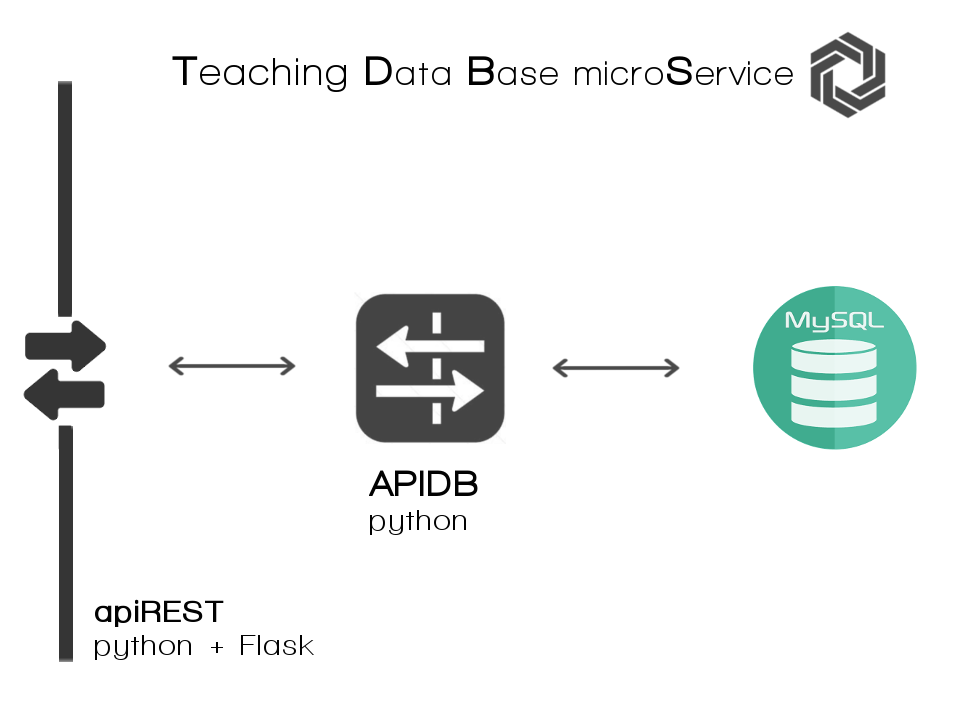
\includegraphics[scale=0.35]{img/graphics/tdbms.png}
\end{center}

\subsubsection{Database logical design}

Based on user histories and the domain of the problem the designe
done based of this entity relation diagram:

The design follow some details that the domain presents, that is related
(at least the more significantly) below:

\begin{center}
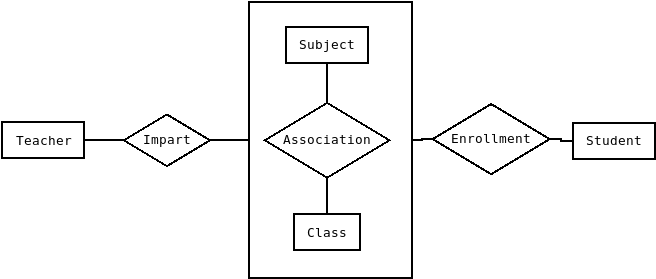
\includegraphics[scale=0.4]{img/diagrams/dbms-ER.png}
\end{center}



\subsubsection{Way to access to raw data}

While at firs of develop the mainly strategie to follow was write
all by cero, finally the point of view has been changed to follow
the use of standard tools and avoid reinvent the wheel.

So, if in the first stages of the project the acces to raw data through
the engine was hand made, using an own simple library that worked
like as simple ORM, the evolution of it and especially the problems
found and the unmaintainability of code have made that now the approach
turned to use a good tool as ORM like \href{http://www.google.es}{SQLAlchemy}.

The changes in the specifications of the api while the develop and
the maintaince of the performance of the queries when is writed hand
made in raw SQL isn't a good idea. Before the develop of this mService
it easy to understand that only in few projects is justified the use
of raw sql sencences and drivers whiout ORM (by easy that it was).


\section{Students Control microService}

\subsection{Domain and design}

\begin{center}
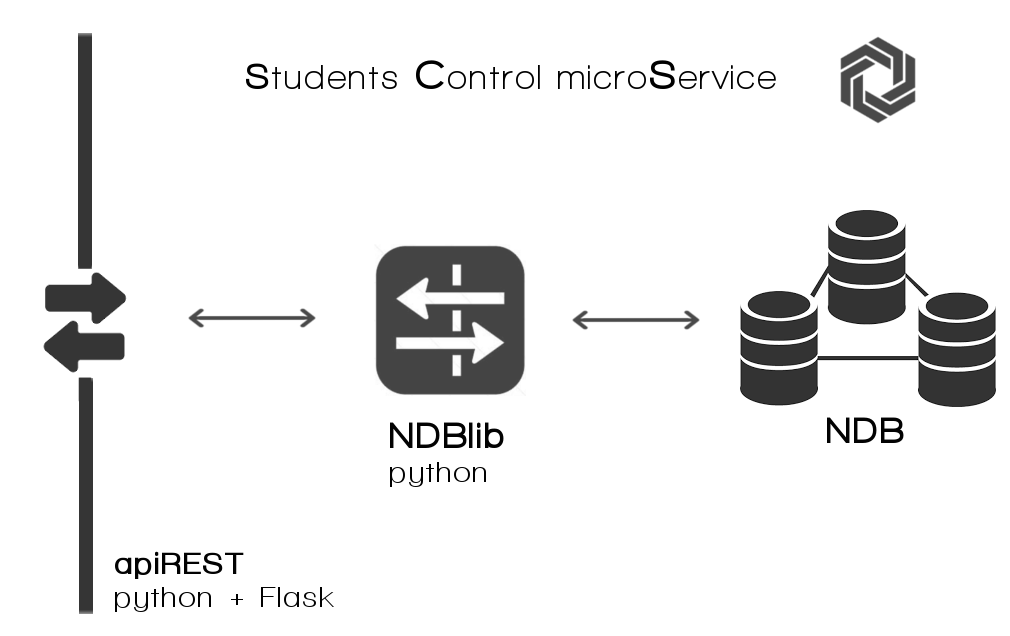
\includegraphics[scale=0.4]{img/graphics/scms.png}
\end{center}

\subsection{Api definition}

skjsñdf
asflkafkdafldañfdsfl


\subsubsection{Attendance Controls Subsection}

This is a simple collection behaviour resource.

This is a RAML0.8 definition file:

\begin{lstlisting}[language=python,frame=none]
  /ac GET POST
   Description:


  /ac/{ac_id} GET PUT DELETE
   Description:


  /ac/base/{ac_id} GET
   Description:
\end{lstlisting}







\section{Analysis microService}

\begin{center}
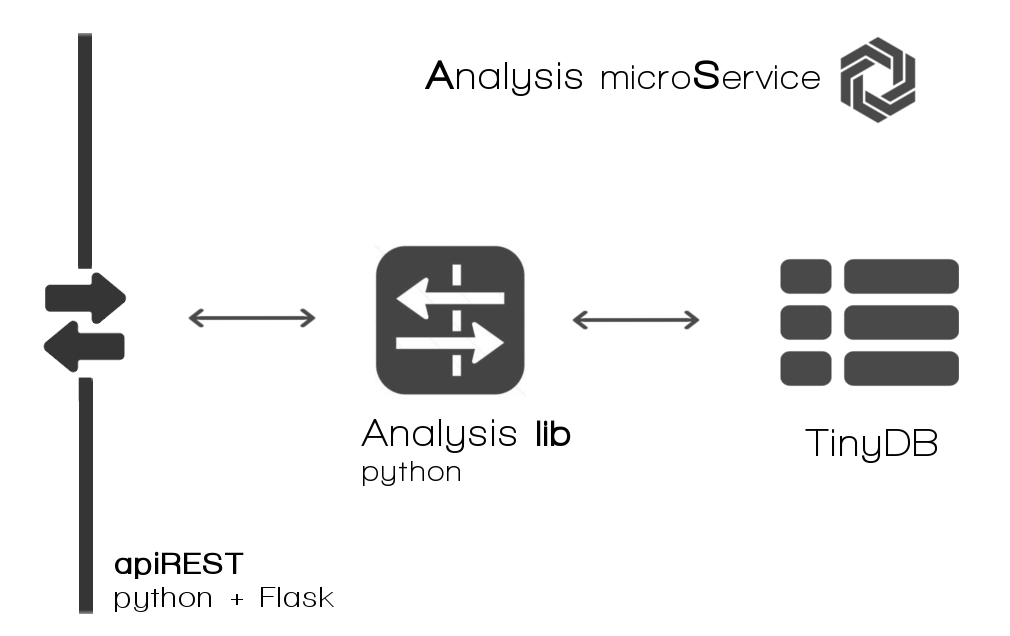
\includegraphics[scale=0.4]{img/graphics/ams.png}
\end{center}

%
\chapter{Develop}

As talk about all details that are been solved or managed would take hundred of
pages in this section we only are going to revise some part of developing that
are been interesting or have required some bit specific design or decision process
and are interesting to explain.

\section{Api Gateway microService}

As was discussed above, the principal goal of this service is to offer the
abstraction of the whole system, so it will not be very complex because all
functionality is actually implemented when this service is built.
\intro
Their unique task is to receive the requests, to construe this and do the call
to the service that must answer it and return the data,
maybe modified.
In common case and in the point of the develop are the service only
reply the queries and return the responses without more logic interaction, but
in the future, this is not only that this will do, because is the perfect place
to implement authorization and authentication with ACLs\footnote{ACL of Access Control List
specifies which users or system processes are granted access to objects, as well
as what operations are allowed on given objects} exploiting the fact that through
this service all calls go.
\intro
Another situation which this service would transform the response of a service or
compound a response with the response of few of them is when must be offered a
resource that is the composition of data arising from several services. For example,
when a user profile info is required, the call will be redirected to Teaching Data
Base mService that will return a simple data block. So, this data block does not
have the image of the user, because this is stored in another different service.
Now the role of gateway take sense because will be it who will retrieve the image
from other service, will insert it in the data block (by some way) and will return
the data block complete.
\intro
It also provides some possibilities to have a dynamic and not locking develop process.
How? Easy, because at first the images can be extracted in execution time from some
library that put example images (or something like this) without locking the APIGmS
and also UImS and so, this service of data storage could be developed after, in another
phase of priorities. So, one more time, the architecture help us to develop team domain
based without any blocking.


\subsection{Cloud Endpoint spike}

As we are working with GAE and GCE the first approach is use
their technology, and if in any resource that you can read about this
they are talking about Google Cloud Enpoints must be some good reason.
This technology is based of an own version of RPC protocol developed
by Google and used in their own intern architecture, called gRPC.
\intro
Basically is another implementation of a Remote Procedure Call
system, but according to Google, really fast and nice, and is true, but has some
drawbacks as for example that can you select other common technologies, as in
our case.
\intro
This is an example of the spike related, it can see in the first phases of the
project.

\begin{lstlisting}[language=python,frame=none]
...

import endpoints
from protorpc import messages

...

class Alumno(messages.Message):
  nombre = messages.StringField(1)
  apellidos = messages.StringField(2)
  id = messages.StringField(3)

class ListaAlumnos(messages.Message):
  alumnos = messages.MessageField(Alumno, 1, repeated=True)

...

@endpoints.api(name='gateway', version='v1')
class GatewayApi(remote.Service):
  """Gateway API v1."""

  @endpoints.method(message_types.VoidMessage, ListaAlumnos,
                    #path=nombre del recurso a llamar
                    path='alumnos/getAlumnos', http_method='GET',
                    #Puede que sea la forma en la que se llama desde la api:
                    #response = service.alumnos().listGreeting().execute()
                    name='alumnos.getAlumnos')

  def getAlumnos(self, unused_request):
    ...
    students_list = []
    ...
    # Logic to get the students list from another service with maybe more logic.
    ...
    alumnosItems.append(Alumno( id=idAlumno, nombre=nombreAlumno.decode('utf-8'), apellidos=apellidosAlumno.decode('utf-8') ) )
    return ListaAlumnos(alumnos=alumnosItems)
...
\end{lstlisting}

\noindent This is only an example, but the complete file has about 2000 lines in the first
approximation of the service.
Now take a look to the \emph{Flask} version, an example bellow,  having exactly
the same functionality of previous code segment.

\begin{lstlisting}[language=python,frame=none]
@api_gateway.route('/students', methods=['GET'])
def get_students():
    ...
    students_list = []
    ...
    # Logic to get the students list from another service with maybe more logic.
    ...
    return students_list
\end{lstlisting}

\noindent The reasons to select Flask insetead of it?
Is not necessary define the schema of the objects, this is sufficient reason
to dismiss their use, but sound enough nice to considere to another
applications in the future (as almos any technology researched).


\subsection{As a simple dispatcher}

This is an example of the behavior dispatching a simple request and answering
exactly the same response from the service.

\begin{lstlisting}[language=python,frame=none]
  @tdbms_segment_api.route('/entities/<string:kind>', methods=['POST'])
  def post_entity(kind):
      response = requests.post(url='http://' + str(modules.get_hostname(module='tdbms')) + '/entities/' + str(kind),
                               json=request.get_json())
      response.headers['Access-Control-Allow-Origin'] = "*"
      return make_response(response.content, response.status_code)
\end{lstlisting}


\begin{lstlisting}[language=python,frame=none]

  @tdbms_segment_api.route('/entities/<string:kind>', methods=['GET'])
  def get_entity(entity_id):
      ...
      response = requests.get(url='...', json=request.get_json())
      ...
      response['profile_image'] = requests.get(url='filesServicesUrl...')
      ...
      return make_response(response, 200)
\end{lstlisting}

\noindent And the next natural step will be built a library that works as a general
customer of any service in the system, to be used in any place where be needed
make a call to any service. This will to work loading dynamically at execution
time the api of each service to know what resources are available and turned
this as Python methods.


\begin{lstlisting}[language=python,frame=none]

  @tdbms_segment_api.route('/entities/<string:entity_id>', methods=['GET'])
  def get_entity(entity_id):
      ...
      response = service['teachingDBmS'].getEntity(entity_id)
      ...
      response['profile_image'] = services['filesStorage'].get(file_id)
      ...
      return make_response(response, 200)
\end{lstlisting}

\noindent With this new tool, the code of the whole project will be reduce 10\% at least.

\section{Teaching Data Base microService}

The deploy of this service is very easy, only has been wrapped the SQL language
in a kind of own ORM, that would be changed by SQLAlchemy as soon as possible in
the next iterations of the project but that is enough for us now. So, instead of
explaining how it is done (it can see in the code of the project) we are going to
explain the more sensible parts and problem detected, to avoid extend too much this
 work.

\subsection{Optional subjects, the ``class'' Table.}

In the domain of the problem can be exists optative subjects and is
needed search a way to implement this because has a specific details
that aren't like the rest.
\intro
The studies plan forces in certain courses to select one or several
optional subjects. For example, if a student has enrollment in 2ºESO
(independently of the group, A, B...) the law and consequently the
studies plan force to the student to choose between some optional
subjects. So, maybe this subjects exists only in this optional case
as \textit{"rare subjects"} but in other cases this are only normal subjects
but that in this course are offer like optional.
\intro
A simple example of this is French subject, it in some courses like
3ESO and 4ESO is obligatory but it in Bachiller (the upper level)
is optional because the students can be select if they want make the
final exam with this second language or select another like English
or Greek or Latin p.e.
\intro
To obtain this we decide develop a simple solution without change
the original database logic schema. So, how we have an entity that
save the classes and it have three attributes, course, word and level
mainly we going to add three more to this special cases, optative,
groupNumber and subgroupNumber. Like this special cases haven't word
param when they have value word don't have and when the item have
word (A, B, C...) then don't have this special attributes.
\intro
Maybe this don't be the best solution, but is a simple in the point
of develop.
Obviously like we can't have two autoincrement values in the same
table definition in MySQL we will need control this programatically,
but is something that we can assume to get our goal easily.But we found a problem.
\intro
The same advantage that offer \textit{UNIQUE} to deleted cases now is problematic
here. While there works fine because this clausulo does not include to items that
have fields to null and allow to exists without conflict in this case if we saved
a optative group obviously would to be \textit{"WORD"} field to null, and if we
do this we can have two groups exactly equals, for example:

\begin{lstlisting}[language=python,frame=none]
1 <null> ESO 1 1 1 0
1 <null> ESO 1 1 1 0
\end{lstlisting}

\noindent This could happens wihtout conflict, and this should be impossible.
For this reason we decide to use the same field \textit{WORD}, with a special
naming, because this never will be used by general groups, that help us to
specify that the group at issue is an optative and also specify the group
and subgroup.
\intro
This is someting like this: OPT\_n\_m
Where \textit{n} will be the group number (must be increased handmade) and \textit{m}
the number of the subgroup (also increased handmade).
Obviously this is only a simple approach to a first solution, will be improved
in next iteration of the service, and we always follow the same philosy,
we prefer explicit way to do something ar implicit, more understandable by
any new developer.
\intro
This way to solve this problem with MySQL engine presents some problems.
As all is managerd by mysql but there are not way to do this automatically
with the own mechanism of myql is necesary to create some distpacher to the
inserction and the deletion to maintain the consistency. When a new optative group
is introduced must be checked that exist the previous (group and subgroup, can not
exists group 4 if 3 does not exists), and the same way should not be possible
delete the group 4 if the number 3 exists yet.
\intro
Note that is important understand that a lot of detail of consistency control
can be relegated to UI, because although there is not allowed by the logic
of interaction from the API must not be allowed neither, to prevent
inconsistencies malicious induced.
\intro
Becuse of this not only the security, also the consistency must be ensured in
any action that user can do.


\section{Students Control microService}

In general terms, this service follows the same philosophy of the rest, with the
difference that they use the Cloud Datastore. In general terms, this service follows
the same philosophy of the rest, with the difference that they use the Cloud Datastore.
That only means that the library of access to raw data is different and instead of
wrap the SQL language as in the last, here we wrap the access to a library designed
by the Cloud Datastore service called \textbf{ndb}, designed by the same Guido Van
Rosum (in the time when worked at Google).
\intro
Most characteristic here is that we need to define the form of the data that we
want to save (this is a heavy reason to do not use again this system, we will
comment this a bit more after).
So, to can store the disciplinary note item type, is necessary to define a
class which ndb can manage it.
\begin{lstlisting}[language=java,frame=none]
  class DisciplinaryNote(ndb.Model):
      # Related academic info.
      studentId = ndb.IntegerProperty()
      teacherId = ndb.IntegerProperty()
      classId = ndb.IntegerProperty()
      subjectId = ndb.IntegerProperty()

      # Disciplinary Note
      kind = ndb.IntegerProperty()
      gravity = ndb.IntegerProperty()
      description = ndb.StringProperty()
      dateTime = ndb.DateTimeProperty()

      # Item Metadata
      createdBy = ndb.IntegerProperty()
      createdAt = ndb.DateTimeProperty()
      modifiedBy = ndb.IntegerProperty(default=None)
      modifiedAt = ndb.DateTimeProperty(default=None)
      deletedBy = ndb.IntegerProperty(default=None)
      deletedAt = ndb.DateTimeProperty(default=None)
      deleted = ndb.BooleanProperty(default=False)
\end{lstlisting}

\noindent And using this denition is builded a wraper to interact, this is
an example of this same section:

\begin{lstlisting}[language=python, frame=none]
  @classmethod
    def post_dn(cls, disciplinary_note):
        if cls.validate_dn(disciplinary_note):
            dn_to_save = DisciplinaryNote(
                studentId=disciplinary_note.get('studentId'),
                teacherId=disciplinary_note.get('teacherId'),
                classId=disciplinary_note.get('classId'),
                subjectId=disciplinary_note.get('subjectId'),
                dateTime=datetime.datetime.strptime(disciplinary_note.get('dateTime'),"%Y-%m-%d %H:%M"),
                kind=disciplinary_note.get('kind'), gravity=disciplinary_note.get('gravity'),
                description=disciplinary_note.get('description'), createdBy=1, createdAt=time_now())
            key = dn_to_save.put()
            return {'status': 200, 'data': {'disciplinaryNoteId': key.id()}}
        else:
            return {'status': 400, 'data': None, 'log': None}
\end{lstlisting}

\noindent With their API resource in Flask:

\begin{lstlisting}[language=python, frame=none]
  @disciplinary_notes_api.route('/disciplinarynote', methods=['POST'])
  def post_disciplinary_note():
    return process_response(DisciplinaryNotesManager.post_dn(request.get_json()))
\end{lstlisting}

\noindent Actually is very simple, the rest of behavior follow the same pattern,
and the only benefits that have the time spent in learning to build the service
with this technology is the amazing performance and cost that store data here has.

\section{User Interface microService}

\subsection{Save processes flows}

The logical process of saving data is apparently easy but it hides some details
when we talk about update existing data. These and how to solve the problem that
it presents will define how the user will use our interface. And spite of this is
a design phase issue is in the develop moment when this appeared and is why it
is explained here.
\intro
Focused on the problem, we have an object load in the interface, as a complete
profile info of a student, and we want to update their data (change or add some
new data) and this is not trivial because will define the signature between the
API of service and the user interface.So, basically, we have found three ways to do this so we are going to analysis
each one to choose the best, even though there are combinations.
When the object is loaded in our interface we modify some field and push the save
button if all the form requirements are satisfied then the complete object is sent
without any else requirements.

\begin{enumerate}
\item \textbf{Common save button}

The object is sent always, independently if it really has suffered changes.
Save button is always available while the requirements of the form are satisfied.

\textbf{Disadvantages}:
The object is always sent, even if is not necessary because it has not suffered
changes, hence a lot of bytes will be sent without sense.

\textbf{Advantages}:
Is the simplest and faster implementation for the user interface and the server
do not need to check anything
only override the object updating their metadata.

\item \textbf{Automatically saved}

The object is sent each time as it suffered any change,
save button not exists. Their behavior is similar to an online text editor where
all changes are saved implicitly.

\textbf{Disadvantages}:
The calls needed are huge if the user to do a lot of changes. Is necessary another
parallel mechanism to maintain the possibility to do undo because if all changes
are saving at the moment in the server there are not any way to do a simply undo action.
A number of calls needed are huge.

\textbf{Advantages}:
Is really futurist because the user does not to need to push any button after of
update their data. All forms become more clear.

\item \textbf{Totally checked}

Is a more efficient way that the rest. In this case, when the object is loaded
in the interface a copy is done and
saved also, always, independently of the interaction of the user. With this, we
achieve to get a copy of the object without any modification when the user is updating some field.

So, each way that user change some field of the form the logic check if there are
any difference between both objects (original copy and the modified) and only
when this difference exists and the requirements of the form are satisfied the
save button will change to enable.
This way if the user cancels the update of the object or after of thousand
modifications leave the object exactly with the same data the send button will
not enable because there are not any to update in the server.

\textbf{Disadvantages}:
The computing requirements in the user device it will high because it will be
needed hundred of checks in a simple interaction.

\textbf{Advantages}:
The server is not involved until the object is really updated. It supposes a user
 experience that gives to interface more intelligent aspect.
\end{enumerate}

\noindent As is easy to imagine the option chosen is the third because the reason explained
above. Down below is shown a piece of code which we have developed the feature of object copy.
When we can to see how is used a variable to save the state of the object, after
the object is saved and watches is enabled with it to detect any possible change
that will modify the state of save button, all after of the student object has been returned.

\begin{lstlisting}[language=java,frame=none, title=studentProfile.js]
...
function loadData() {
    vm.student = StudentsService.get({id: vm.studentId}, function () {
        ...
        vm.studentOriginalCopy = angular.copy(vm.student);
        $scope.studentModelHasChanged = false;
        $scope.$watch('vm.student', function (newValue, oldValue) {
            $scope.studentModelHasChanged = !angular.equals(vm.student, vm.studentOriginalCopy);
            if ($scope.studentModelHasChanged)
                vm.updateButtonEnable = true;
            else
                vm.updateButtonEnable = false;
        }, true);
    }, function () {
        console.log('Student not found')
        ...
    });
    ...
}
...
\end{lstlisting}

\noindent So, this behaviour is replied in all places where this kind of interaction appears.
\intro
Another important thing to design is the interaction between the differents parts
of the interface. The menus, buttons and the flow among these can be the difference
between a good and bad application because, at this time, there are few things
that do not exists, but between the existing, a good UI/UX in one of two similar
apps can be enough to triumph.
\intro
In our case, all interactions are well-defined, trying to build a simple and
powerful user interface. This is an example of the interaction flow that defines
the processes to add some teaching to a teacher.
This is only an example, we could fill dozens of pages with flow diagrams, but
we think that it is enough representative.


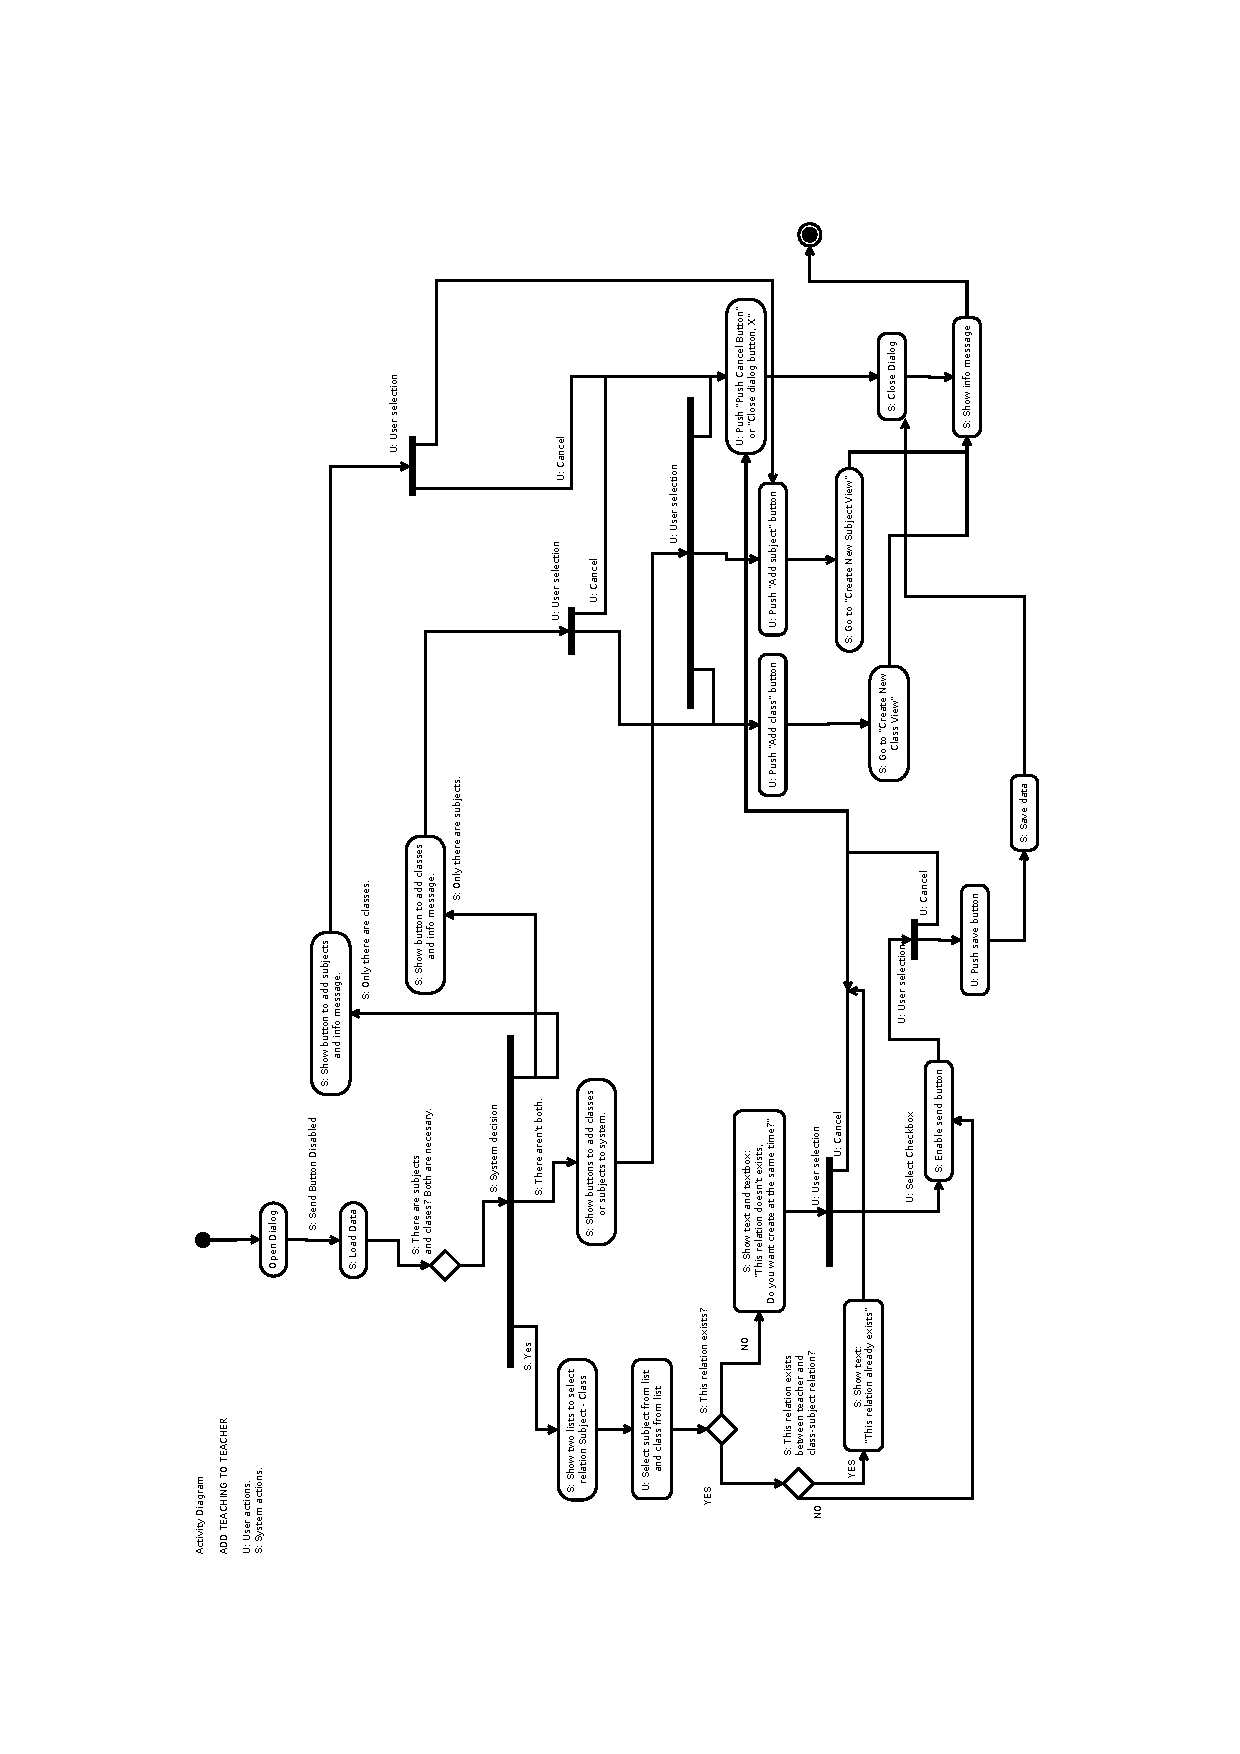
\includepdf[pages=-,pagecommand={},scale=0.94]{img/diagrams/addTeachingToTeacher_AD.pdf}

% \begin{figure}[H]
%   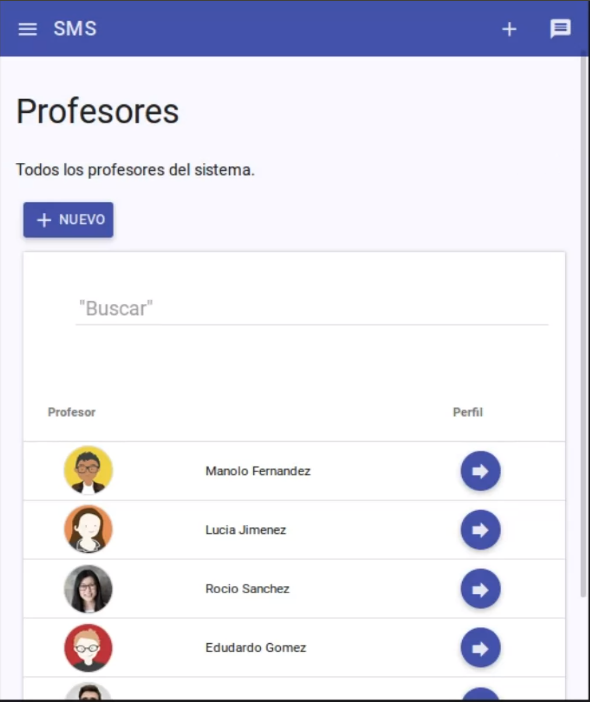
\includegraphics[scale=0.2]{img/snaps/teachers_list.png}
%   \centering
%   \caption{Teachers List view wireframed.}
% \end{figure}
%
% \begin{figure}[H]
%   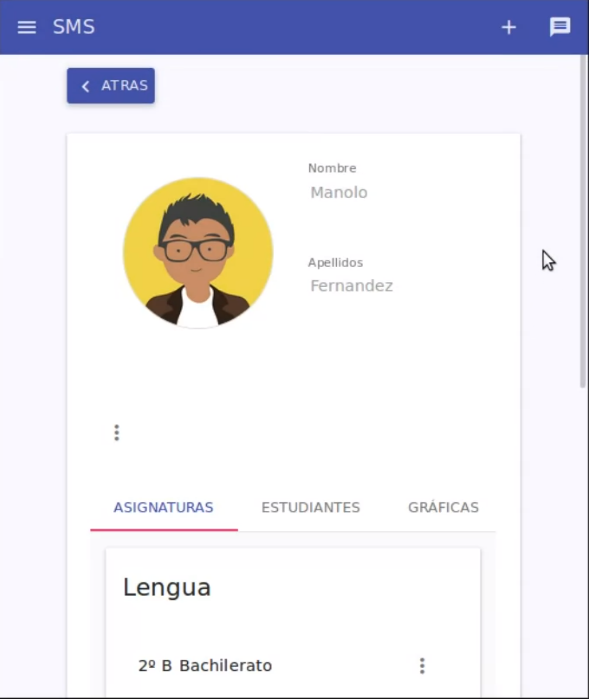
\includegraphics[scale=0.2]{img/snaps/teacher_profile.png}
%   \centering
%   \caption{Teachers List view wireframed.}
% \end{figure}

\noindent One has been decided the design with wireframes and the interaction
with flow/activity diagrams the rest is to implement this with CSS Framework
selected and develop all logic so the system satisfies all requirements.
This is some snaps of the interface already designed.
\intro
The teacher list, where we can see a simple dynamic list to manage teachers,
where we can see basic info and can access to complete info. And can see the
material design rules applied already.

\begin{figure}[H]
\centering
\begin{minipage}{.5\textwidth}
  \centering
  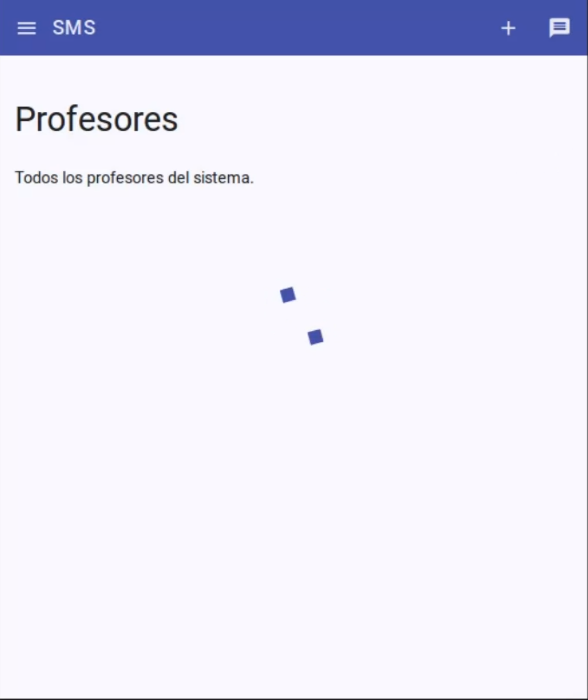
\includegraphics[scale=0.3]{img/snaps/teachers_list_preload.png}
  \caption{Teachers list loading.}
\end{minipage}%
\begin{minipage}{.5\textwidth}
  \centering
  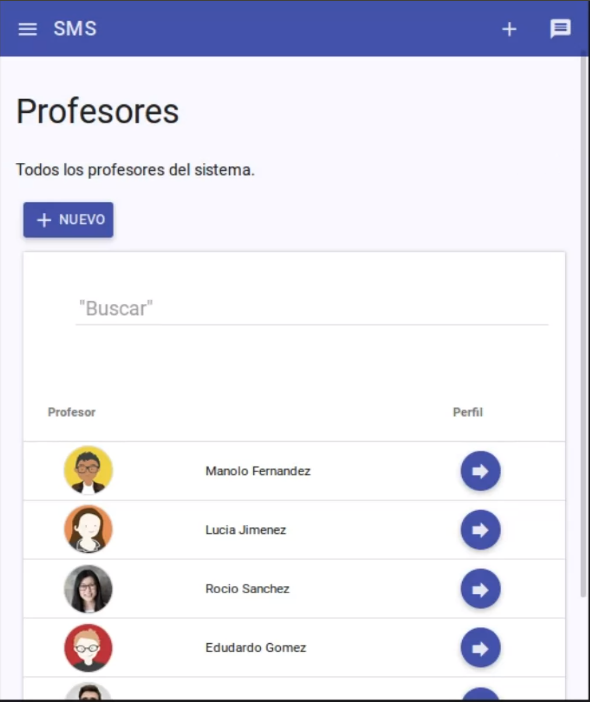
\includegraphics[scale=0.3]{img/snaps/teachers_list.png}
  \caption{Teachers list loaded.}
\end{minipage}
\end{figure}

\noindent The pictures below show us teacher profile section, with
the same philosophy.

\begin{figure}[H]
\centering
\begin{minipage}{.5\textwidth}
  \centering
  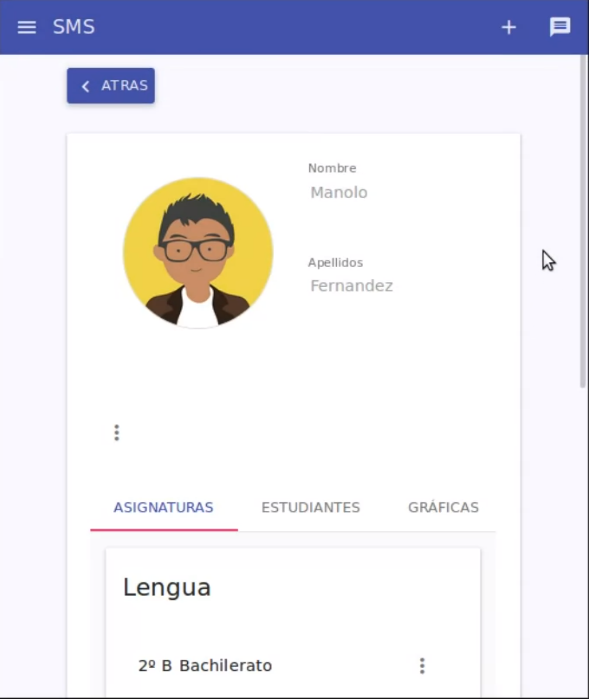
\includegraphics[scale=0.3]{img/snaps/teacher_profile.png}
  \caption{Teacher profile.}
\end{minipage}%
\begin{minipage}{.5\textwidth}
  \centering
  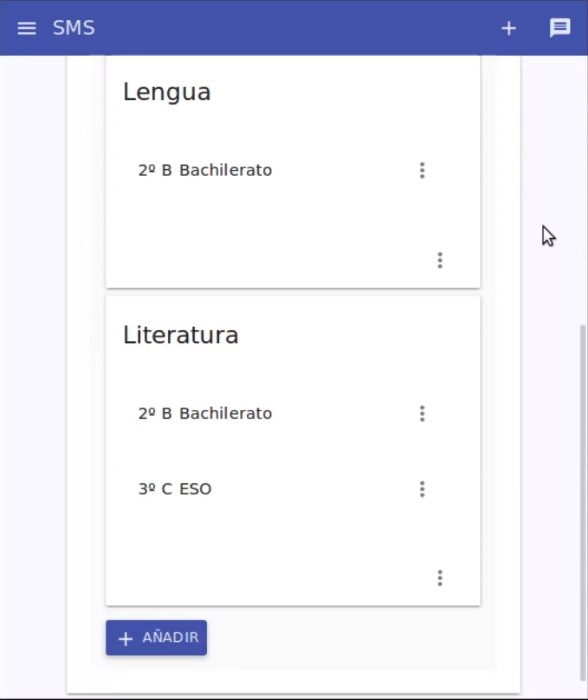
\includegraphics[scale=0.3]{img/snaps/teacher_profile_2.png}
  \caption{Teaching section.}
\end{minipage}
\end{figure}

\noindent Aso, for example, updating a teacher profile (note that this is
the spanish version).

\begin{figure}[H]
\centering
\begin{minipage}{.5\textwidth}
  \centering
  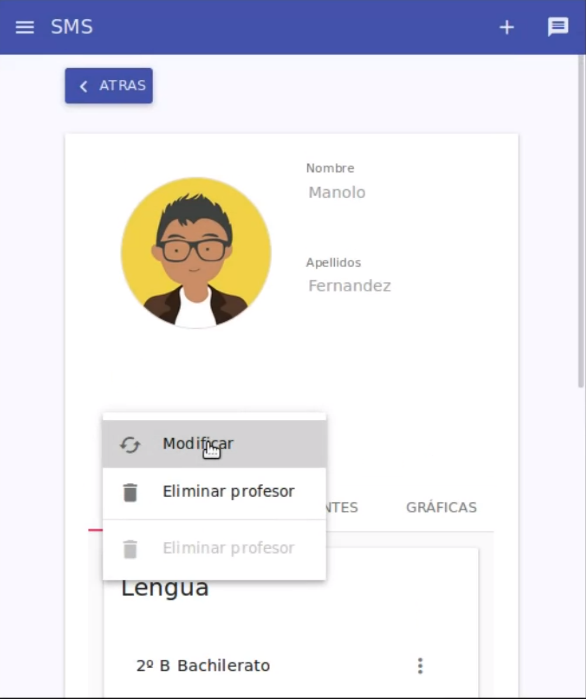
\includegraphics[scale=0.3]{img/snaps/teacher_profile_update.png}
  \caption{Updating a teacher.}
\end{minipage}%
\begin{minipage}{.5\textwidth}
  \centering
  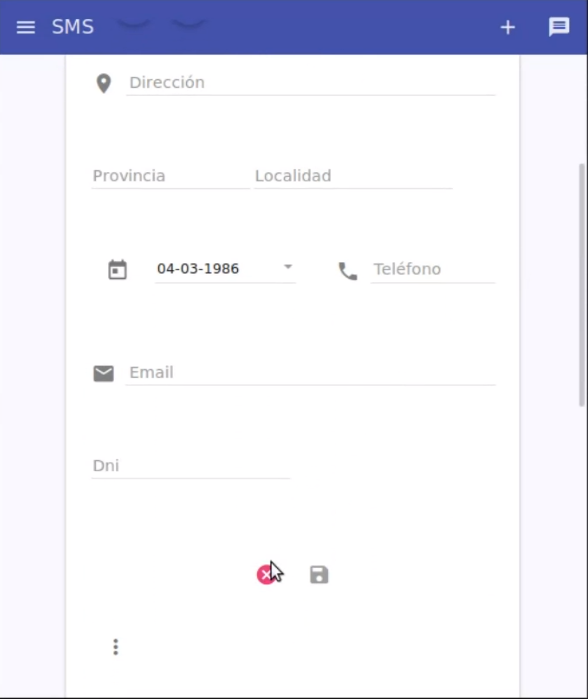
\includegraphics[scale=0.3]{img/snaps/teacher_profile_update2.png}
  \caption{Fields hidden.}
\end{minipage}
\end{figure}

\noindent Now, students list view and some graphics.

\begin{figure}[H]
\centering
\begin{minipage}{.5\textwidth}
  \centering
  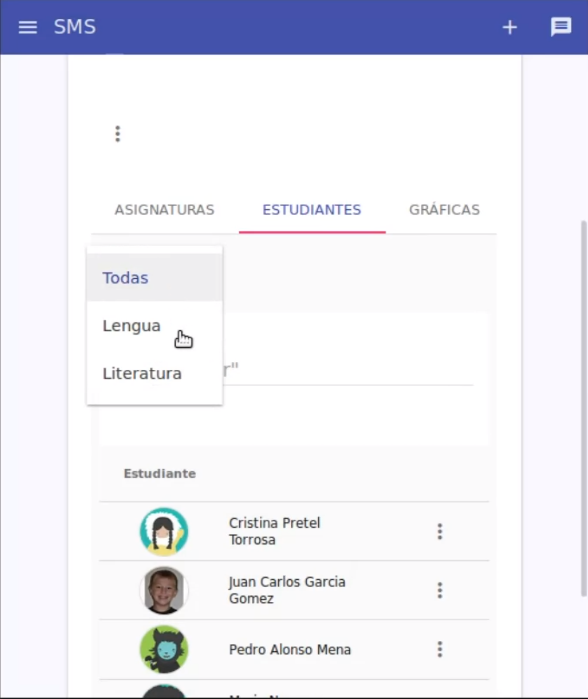
\includegraphics[scale=0.3]{img/snaps/teacher_profile_students.png}
  \caption{Students list.}
\end{minipage}%
\begin{minipage}{.5\textwidth}
  \centering
  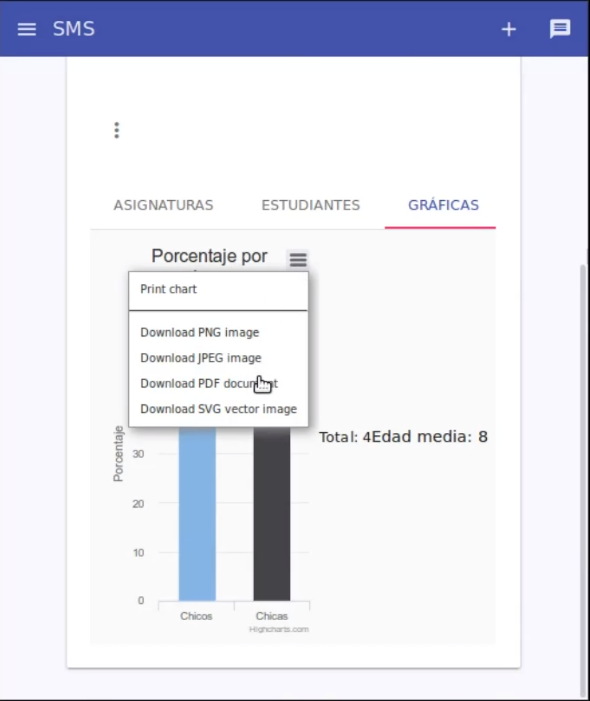
\includegraphics[scale=0.3]{img/snaps/teacher_profile_graphics.png}
  \caption{Students simple report.}
\end{minipage}
\end{figure}

\noindent And the rest of app follow the same look and feel, responsive and well adaptable
for almost any device.

\section{Analysis microService}

In the case of this service, the developing not have gone too far and only have
been implemented some simple linear regressions to can give a simple way to
predict the future values of some data block, as student marks or their efficiency
(as we have discussed already).

In conclusion, this service will offer mocks of all data expected and will be
the main goal in futures sprints of the project.

%
\chapter{Conclusions}

Only a few months might not sound much but is enough to obtain some
conclusion about techonologíes, patterns and ways to develop.
\intro
This work can not finish without a reflexion about what have been the mainly
drawbacks and locks in the develop, design and evolution of the entire project,
trying to propose solutions and overall, learning a lot about all.

\subsection{Scheduling}

The scheduling of development is very easy to do, in the hypothetical case that
all goes fine, but as is normal, there are a lot of factors hard to control that
besides are unknown at the beginning.
\intro
If we join this with an inexpert scrum master and technologies absolutely new for
the team (without a good spikes issues to select and try these) the result can
be catastrophic.
\intro
If we remember the planification that we did in the chapter three, we had estimated
the project in 6 months, that was equeal to 12 sprints, and when them finished
the project would be finished, as can see in the graphic.

\begin{figure}[H]
  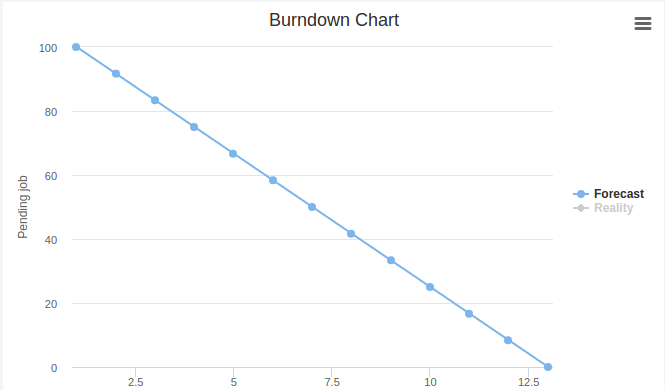
\includegraphics[scale=0.45]{img/graphics/burndown.png}
  \centering
  \caption{Project forecast.}
\end{figure}

\noindent The problem is that the develop has not passed as we would have liked,
and, without going into too much detail, after of our auto evaluation and
evaluation of the sprints and the work that has been finished we can say that
only is finished approximately of 50\% that we expeted to be a stable first version
that we can put in production.
You can see the values in the next graphic.

\begin{figure}[H]
  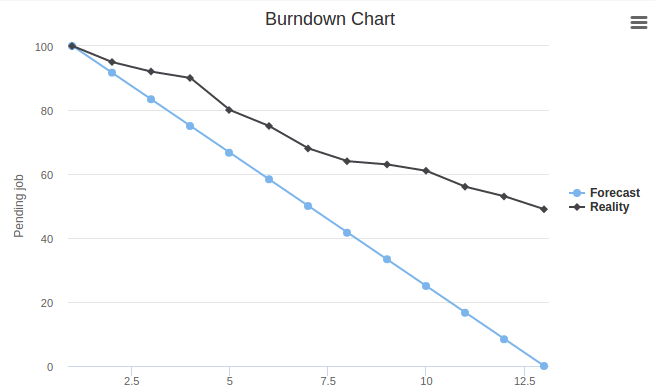
\includegraphics[scale=0.45]{img/graphics/burndown2.png}
  \centering
  \caption{Project forecast and reality.}
\end{figure}

\noindent Obviously, if the project continues, it would need a lot of
modifications and analysis to detect fine-grained which are the reasons
of the 50\% of delay, in addition to those already detected here,
because doing an estimate of the time that at this rithm the project would required
without any modification in the process of production we have that we would need
around 25 sprints, that means another 6 month of develop.

\begin{figure}[H]
  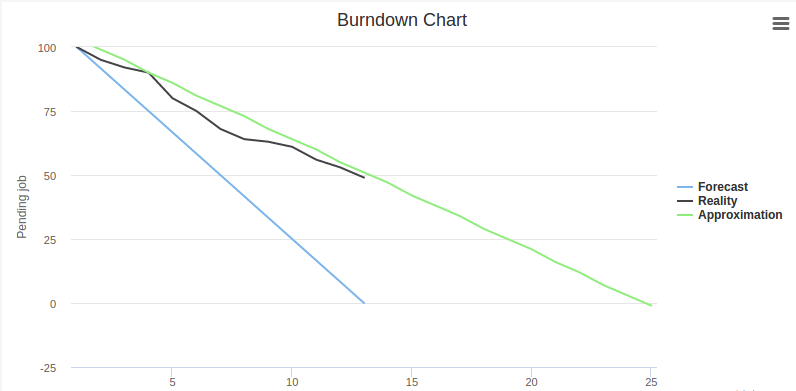
\includegraphics[scale=0.45]{img/graphics/burndown3.png}
  \centering
  \caption{Burndown chart with plannig, workd done and prevision to deadline}
\end{figure}

\noindent These are not good news, the double of time means the double of resources (time and
money) and loose customer confidence, some that we never can not lose.
Despite this, for our feeling, and talking about an pseudo academic work,
the result is not as wrong as could be, and with all predictable fails,
it has not been a bad finish. Knowing that this kind of things only can happens
one time, and should be use to lear and to avoid to make the same mistakes.
\intro
And if we should be do the same project again, our provision would be other
very different, planning exactly the same issues, we calculate that could be
that in less of a half of time, as this forecast shows.

\begin{figure}[H]
  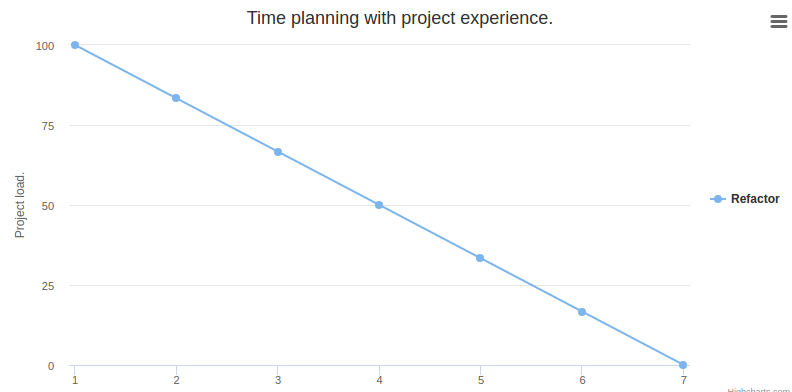
\includegraphics[scale=0.4]{img/graphics/redo.png}
  \centering
  \caption{Replaning experience based.}
\end{figure}

\subsection{Technologies and frameworks}

Of one side, we have the difficulties with the technology choice. In this case
can be said that use AngularJS and Python has been literally perfect, beyond
that the typical novice errors with the languages and their learning curves.
So, in general, without a doubt, they will be chosen as technologies again.
\intro
About the platforms or technologies the point of view changes. If you are
an expert developer using platforms like Google App Engine can be really
interesting, because you are evaluated the rest of the options, but when
you don't have any practice, in my view, is not a good option. Moreover when
the learning curve is so soft.
\intro
As in many new technologies is easy to do the first steps, but develop some bigger
is another thing, especially when we are not talking about frameworks and
languages standard as C++, Java or PHP. So, before to select one is really justify
the spike of some of these.
\intro
About the API frameworks, Flask was a good selection, because their ease of use
and lightness does it perfectly. However, when we analyze the performance, there are
other solutions also in python faster. An example of this is Falcon\footnote{Defined as: \textit{"A
very fast, very minimal Python web framework for building microservices, app backends,
and higher-level frameworks"}. More info at: \textit{falconframework.org}}. As can be
seen in the next picture, extracted from py-frameworks-bench\footnote{
http://klen.github.io/py-frameworks-bench/} project, we can see how Falcon has
better performance than Flask. In this graphic is measure the response in ms
of encode an object to JSON and return the response.

\begin{center}
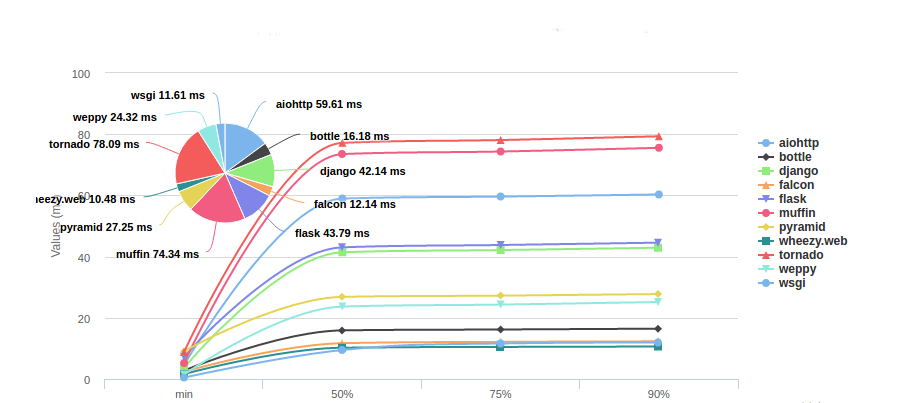
\includegraphics[scale=0.5]{img/graphics/frameworks.png}
\end{center}

\noindent And Falcon would be our selection today (even more having some practice in
company).
\intro
About Sphinx, is a good choice, but it has something that could be improved and
is the requirements of that the project must have. To use Sphinx your project
needs to be \textit{executable}, understanding this as all imports must work.
Many people do not know why Sphinx have this restriction, so if you
only want doc, independently of if you structure is correct or not, well, this is
impossible in the actual version, we hope that change this at any moment.

\subsubsection{About the platform}

In spite of Google App Engine is a good tool it has some drawbacks that some are
very obvious at first and others that can go unnoticed until you are working with it.
the sandbox restrictions as use python only in their version 2.7 at first is not
a problem but when you discover that the most of the libraries that you need works
better in 3.x, or some are deprecated in 2.7, out of maintenance is not a good
signal, especially when you have some block and the help of community is focused
on upper versions. It happened in the standard version of App Engine sandbox, to
solve this the team of it launched App Engine Flexible Environment, where you can
run any code but the configuration is not trivial and it although is configurable by
docker file is a strange mix between the auto maintained and scalable isolated
sandbox and the standard containers developer managed.
\intro
So, taking advantage of all services of the infrastructure of GCE, another
architecture that we will develop in the future will run only into docker containers,
using the services required (SQL, DataStore or another and running over compute layer,
not with google app engine.

\subsubsection{About the database}

About database, without doubt, MongoDB is nowadays the better solution that
can be used in a project with low relational requirements, because their learning
curve is so good that is easy to have a good prototype of database layer soon,
and the resources of the community greatly assist.

\subsection {Design}

\subsubsection{About the user interface}

There are any that has been critical in the develop and is that the assumption
as a good idea that all interface always is loaded when a user enters to the app,
but after some tests have been seen that is not the best way.  For this reason,
many teams that work with Angular choose an alternative, use a library specially
designed to load the javascript files of the app needed in each part of the interface.
\intro
So, if a user is in the teaching section don't need all files of the reports section, and this files only will be loaded when the user insert in this section. To do this,
the teams use the Require.js\footnote{Literraly from their website ,requirejs.org: \textit{"RequireJS is a
JavaScript file and module loader. It will improve the speed and quality of your code."}} library as
the standard dynamically loader and their use will be the next step to do the
load of the app faster.
\subsubsection{About the compression of APIs}

Is easy to notice that the API of Students Control microService is very semantic
but very big also (become more complex to maintain and change) while of the
teaching service API is very compact and little but less semantic, because the
meaning of their resources is not clear and therefore their behavior neither.
It was made on purpose it to check in the development which approach was more
problematic or simple to explain or update.
\intro
And the conclusion is that to maintain the coherency between the domain drive
development of the service and the expressivity of the API the customers do not
need to know the internal work of the service, but need understand the logic
behind of the items, so, in the future, it will be moved to an approach more human
readable (in spite of all disadvantages, talking about code and maintenance).

\subsection{The develop process}

Can be really interesting if you use any methodology as SCRUM and the developer's
team work together. But when the team is a single developer and the project only
have sporadic contributions,
all is more difficult to follow. Other techniques can be used but SCRUM, eXPrograming
or something like this not works fine to only one person.
\intro
So, independently, is a good point to start to practice. For another hand, is
noticed that the sporadic contributions as in a Hackathon or in a simple day are
difficult too because, as is normal, the people require a time to understand the
project, the technology and all related with it.

\subsection{Opportunities}

Take part of some software contest is the better decision that any
software student can take. Visibility, networking, new friendship are only some
benefits that can achieve.
\intro
Thanks to enrolling this project of the contests that the Open Source Department of
the University of Granada with JJ Merelo as principal organizes was offer a job
in a related software company with the technologies and patterns used.
So, if any people think that the participation, the contribution, and involvement
is not useful, is absolutely wrong. In all cases, this attitude front the
students only return benefits.

\subsection{Future of the project}

At the beginning of the develop, the idea behind of this was put in production
the result in a few months in beta mode in a school center of Granada, but now,
the jobs opportunities referred above have been done that the project go to the
another plane, less important, because the ideas and the philosophy are
developed just now with another really good engineers in a company, building a
privative software, architecture, and new related tools.
\intro
So, independently the license of the code has not changed, and the develop can
go ahead with any developer or group of them that want. For another hand the
continuous evolution of the technologies do this issue a
bit difficult, and actually, it is another learned lesson about the innovate
software using three party technologies, we will never have the safety that the
technology never will change. If you are working with C++ or even Java with you
own infrastructure the changes are minimal through the months, with third party
technologies and support you need be at day with all changes and update almost
all your software each year. So, in this cases is difficult that the continuity
of the project will be ensured, at least without the original designer inside the
new developer's teams. But, anyway, is only a point of view, with the software
nothing can be assumed.
\intro
Independently, the code is open, to learn, to review, and maybe to help someone,
so for this part, we are happy.

\subsubsection{Data processing}

Finally the project has not grow as much as we would have liked, and this part
is not enough powerful to their possibilities. The huge amount of data joined
with their clear relations does this especially interesting to apply techniques
as data mining or machine learning. The simple relations between data is easy
to see but can be exists dozen of interesting relations that can go undetected
and their work will be the mainly task in futures iterations.

\subsection{Open Source}

Other conclusions obtained in the solution development are related to open source and the
viability to survive on this. Many time in the college is easy to hear that the
open source is a good way to start and is true, but not if you want to work of
this. Work in open source projects is really interesting, for the community,
for the workflow, for build some useful to the community and by a huge list of
advantages. But this is possible only when for one hand you are working in a
company and some of the projects of this are decided to be open, independently of the
reason, community, better visibility, etc. or when you are a student and have
the opportunity to free amounts of code, as this case. But for another hand,
thinking to build a company, more o less big based on an open source solution
is very very rare and complex, mainly to younger and inexpert software developers.
\intro
Obviously in the most cases, always there are some exceptions that are
wonderful examples that project with an amazing grow, and a really amount of
code that any developer must have would be open, always open, because there
are any developer that can learn alone, without the community (in any of their
forms) and be in the obligation to contribute, to give back the favor.

\subsection{Closing}
This project has been a great opportunity to learn a lot about amount of things,
but especially about myself, has been another opportunity to know how to deal with
new challenges, how to work a first really subtle approach to project management and
the most important, to know which my bigger faults.
It have helped me to understand that this is only the begin, the beginning of
the way that only can be covered if you do not stop to learn never, absolutely never.
\intro
So, \textbf{let's start!}

%
%
%%\nocite{*}
\bibliography{bibliography/bibliography}
\addcontentsline{toc}{chapter}{Bibliografía}
\bibliographystyle{miunsrturl}
%
\appendix
\newpage
\section{\\Appendix A: User Stories}

This is the list of user stories related with the chapter 2, Requirements.

% General needs User Storie #1 #################################################
\noindent\shadowbox{
\begin{minipage}[t]{1\columnwidth - 2\fboxsep - 2\fboxrule - \shadowsize}
  \begin{flushleft}
    \smallskip
    As user, I want to use the app in any device.
  \end{flushleft}
\break
Aceptance criteria:
\begin{itemize}
\item Must be accesible from:
\begin{itemize}
\item Smartphones
\item Tablets
\item Laptop
\item Standar Computers
\end{itemize}
\item The item must be inserted, readed, updated and deleted.
\end{itemize}
\hrule
\bigskip
\textbf{GN \#1 } - High priority
\end{minipage}}
% ##############################################################################

% General needs User Storie #2 #################################################
\noindent\shadowbox{
\begin{minipage}[t]{1\columnwidth - 2\fboxsep - 2\fboxrule - \shadowsize}
  \begin{flushleft}
    \smallskip
    As user, I want to load in the system data from another databases and formats.
  \end{flushleft}
\break
Aceptance criteria:
\begin{itemize}
\item Must be compatible with formats:
\begin{itemize}
\item XML
\item CSV
\item JSON
\end{itemize}
\end{itemize}
\hrule
\bigskip
\textbf{GN \#2 } - High priority
\end{minipage}}
% ##############################################################################

% General needs User Storie #3 #################################################
\noindent\shadowbox{
\begin{minipage}[t]{1\columnwidth - 2\fboxsep - 2\fboxrule - \shadowsize}
  \begin{flushleft}
    \smallskip
    As user, I want to get the database of the app to migrate if was necesary.
  \end{flushleft}
\break
Aceptance criteria:
\begin{itemize}
\item Must be compatible with formats:
\begin{itemize}
\item XML
\item CSV
\item JSON
\end{itemize}
\end{itemize}
\hrule
\bigskip
\textbf{GN \#3 } - High priority
\end{minipage}}
% ##############################################################################

% Academic Management System User Storie #1 ####################################
\noindent\shadowbox{
\begin{minipage}[t]{1\columnwidth - 2\fboxsep - 2\fboxrule - \shadowsize}
As manager, I want to save students to can to register them.
\break
Aceptance criteria:
\begin{itemize}
\item The item must be this fields.
\begin{itemize}
\item Name
\item Surname
\item DNI
\item Email
\item Address
\item Locality
\item Province
\item Birthdate
\item Phone
\item Image
\item Gender
\end{itemize}
\item The item must be inserted, readed, updated and deleted.
\end{itemize}
\hrule
\bigskip
\textbf{AMS \#1 } - High priority
\end{minipage}}
% ##############################################################################

% Academic Management System User Storie #2 ####################################
\noindent\shadowbox{
\begin{minipage}[t]{1\columnwidth - 2\fboxsep - 2\fboxrule - \shadowsize}
As manager, I want to save teachers to can to register them.
\break
Aceptance criteria:
\begin{itemize}
\item The item must be this fields.
\begin{itemize}
  \item Name
  \item Surname
  \item DNI
  \item Email
  \item Address
  \item Locality
  \item Province
  \item Birthdate
  \item Phone
  \item Image
  \item Gender
\end{itemize}
\item The item must be inserted, readed, updated and deleted.
\end{itemize}
\hrule
\bigskip
\textbf{AMS \#2 } - High priority
\end{minipage}}
% ##############################################################################


% Academic Management System User Storie #3 ####################################
\noindent\shadowbox{
\begin{minipage}[t]{1\columnwidth - 2\fboxsep - 2\fboxrule - \shadowsize}
As manager, I want to save subjects to can to register them.
\bigskip
\break
Aceptance criteria:
\begin{itemize}
\item The item must be this fields.
\begin{itemize}
\item Name
\item Description
\end{itemize}
\item The item must be inserted, readed, updated and deleted.
\end{itemize}
\hrule
\bigskip
\textbf{AMS \#3 } - High priority
\end{minipage}}
% ##############################################################################


% Academic Management System User Storie #4 ####################################
\noindent\shadowbox{
\begin{minipage}[t]{1\columnwidth - 2\fboxsep - 2\fboxrule - \shadowsize}
As manager, I want to save classes to can to can to register them.
\bigskip
\break
Aceptance criteria:
\begin{itemize}
\item The item must be this fields.
\begin{itemize}
\item Course
\item Word
\item Level
\item Description
\end{itemize}
\item The item must be inserted, readed, updated and deleted.
\end{itemize}
\hrule
\bigskip
\textbf{AMS \#4 } - High priority
\end{minipage}}
% ##############################################################################


% Academic Management System User Storie #5 ####################################
\noindent\shadowbox{
\begin{minipage}[t]{1\columnwidth - 2\fboxsep - 2\fboxrule - \shadowsize}


As manager, I want to save relation between subjects and classes.
\bigskip
\break
Aceptance criteria:
\begin{itemize}
\item The item must be inserted, readed, updated and deleted.

\end{itemize}
\bigskip
\hrule
\bigskip
\textbf{AMS \#5 } - High priority
\end{minipage}}
% ##############################################################################


% Academic Management System User Storie #6 ####################################
\noindent\shadowbox{
\begin{minipage}[t]{1\columnwidth - 2\fboxsep - 2\fboxrule - \shadowsize}
  \begin{flushleft}
    As manager, I want to save relation between teachers and the
    relation between subjects and classes.
  \end{flushleft}
\bigskip
\break
Aceptance criteria:
\begin{itemize}
\item The item must be inserted, readed, updated and deleted.

\end{itemize}
\bigskip
\hrule
\bigskip
\textbf{AMS \#6 } - High priority
\end{minipage}}
% ##############################################################################

% Academic Management System User Storie #7 ####################################
\noindent\shadowbox{
\begin{minipage}[t]{1\columnwidth - 2\fboxsep - 2\fboxrule - \shadowsize}
\begin{flushleft}
  \smallskip
  As manager, I want to save relation between students and the
  relation between subjects and classes.
\end{flushleft}
\bigskip
\break
Aceptance criteria:
\begin{itemize}
\item The item must be inserted, readed, updated and deleted.

\end{itemize}
\bigskip
\hrule
\bigskip
\textbf{AMS \#7 } - High priority
\end{minipage}}
% ##############################################################################


% Attendance Controls User Storie #1 ####################################
\noindent\shadowbox{
\begin{minipage}[t]{1\columnwidth - 2\fboxsep - 2\fboxrule - \shadowsize}
As teacher, I want to save attendance of students to can to register them.
\bigskip
\break
Aceptance criteria:
\begin{itemize}
\item The item must be this fields.
\begin{itemize}
\item Attendance
\item Delay
\item Justification
\end{itemize}
\item The item must be inserted, readed, updated and deleted, in a list of
all students of the class.
\end{itemize}
\hrule
\bigskip
\textbf{AC \#1 } - High priority
\end{minipage}}
% ##############################################################################

% Class control User Storie #1 ####################################
\noindent\shadowbox{
\begin{minipage}[t]{1\columnwidth - 2\fboxsep - 2\fboxrule - \shadowsize}
As teacher, I want to save attendance of students to can to register them.
\bigskip
\break
Aceptance criteria:
\begin{itemize}
\item The item must be this fields.
\begin{itemize}
\item Attendance
\item Delay
\item Justification
\end{itemize}
\item The item must be inserted, readed, updated and deleted, in a list of
all students of the class.
\end{itemize}
\hrule
\bigskip
\textbf{CC \#1 } - High priority
\end{minipage}}
% ##############################################################################

% Marks USER STORY n1 #########################################################
\noindent\shadowbox{
\begin{minipage}[t]{1\columnwidth - 2\fboxsep - 2\fboxrule - \shadowsize}


As teacher or educator, I want to record bad behaviour of a student.
\bigskip
\break
Aceptance criteria:
\begin{itemize}
\item The item must be this fields.
\begin{itemize}
\item Course
\item Word
\item Level
\item Description

\end{itemize}
\item The item must be inserted, readed, updated and deleted.

\end{itemize}

\hrule
\bigskip
\textbf{MRKS \#1 } - High priority
\end{minipage}}
% ##############################################################################


% Disciplinary Notes USER STORY n1 #############################################
\noindent\shadowbox{
\begin{minipage}[t]{1\columnwidth - 2\fboxsep - 2\fboxrule - \shadowsize}


As teacher or educator, I want to know most common disciplinary notes and
data related.
\bigskip
\break
Aceptance criteria:
\begin{itemize}
\item The item must be this fields.
\begin{itemize}
\item Course
\item Word
\item Level
\item Description

\end{itemize}
\item bla bla bla.

\end{itemize}

\hrule
\bigskip
\textbf{DN \#1 } - High priority
\end{minipage}}
% ##############################################################################



% Disciplinary Notes USER STORY n2 #############################################
\shadowbox{
\begin{minipage}[t]{1\columnwidth - 2\fboxsep - 2\fboxrule - \shadowsize}


As teacher or educator, I want to record bad behaviour of a student.
\bigskip
\break
Aceptance criteria:
\begin{itemize}
\item The item must be this fields.
\begin{itemize}
\item Course
\item Word
\item Level
\item Description

\end{itemize}
\item The item must be inserted, readed, updated and deleted.

\end{itemize}

\hrule
\bigskip
\textbf{DN \#2 } - High priority
\end{minipage}}
% ##############################################################################



% Simple and A. Reports USER STORY n1 #############################################
\noindent\shadowbox{
\begin{minipage}[t]{1\columnwidth - 2\fboxsep - 2\fboxrule - \shadowsize}


As any person of center I want to have simple and advanced reports about
the state of the student.
\bigskip
\break
Aceptance criteria:
\begin{itemize}
\item The item must be this fields.
\begin{itemize}
\item Change

\end{itemize}
\item bla bla bla.

\end{itemize}

\hrule
\bigskip
\textbf{SAR \#1 } - High priority
\end{minipage}}
% ##############################################################################

% Seneca USER STORY n1 #########################################################
\noindent\shadowbox{
\begin{minipage}[t]{1\columnwidth - 2\fboxsep - 2\fboxrule - \shadowsize}


As a teacher, I need not interact manually with the official system.
\bigskip
\break
Aceptance criteria:
\begin{itemize}
\item The item must be this fields.
\begin{itemize}
\item Course
\item Word
\item Level
\item Description

\end{itemize}
\item The marks of students must be updload automat

\end{itemize}

\hrule
\bigskip
\textbf{SNC \#1 } - High priority
\end{minipage}}
% ##############################################################################

% General needs User Storie #1 #################################################
\noindent\shadowbox{
\begin{minipage}[t]{1\columnwidth - 2\fboxsep - 2\fboxrule - \shadowsize}
As user, I want to use the app in any device.
\break
Aceptance criteria:
\begin{itemize}
\item Must be accesible from:
\begin{itemize}
\item Smartphones
\item Tablets
\item Laptop
\item Standar Computers
\end{itemize}
\item The item must be inserted, readed, updated and deleted.
\end{itemize}
\hrule
\bigskip
\textbf{GN \#1 } - High priority
\end{minipage}}
% ##############################################################################

% General needs User Storie #2 #################################################
\noindent\shadowbox{
\begin{minipage}[t]{1\columnwidth - 2\fboxsep - 2\fboxrule - \shadowsize}
JSON
\break
Aceptance criteria:
\begin{itemize}
\item Must be accesible from:
\begin{itemize}
\item Smartphones
\item Tablets
\item Laptop
\item Standar Computers
\end{itemize}
\item The item must be inserted, readed, updated and deleted.
\end{itemize}
\hrule
\bigskip
\textbf{GN \#1 } - High priority
\end{minipage}}
% ##############################################################################

% General needs User Storie #3 #################################################
\noindent\shadowbox{
\begin{minipage}[t]{1\columnwidth - 2\fboxsep - 2\fboxrule - \shadowsize}
STATUS RESPONSE
\break
Aceptance criteria:
\begin{itemize}
\item Must be accesible from:
\begin{itemize}
\item Smartphones
\item Tablets
\item Laptop
\item Standar Computers
\end{itemize}
\item The item must be inserted, readed, updated and deleted.
\end{itemize}
\hrule
\bigskip
\textbf{GN \#1 } - High priority
\end{minipage}}
% ##############################################################################

\newpage
\section{\\Appendix B: APIs definitions}

\begin{lstlisting}[language=python,frame=none]
  #%RAML 0.8
  title: Teaching Data Base API
  version: 1.0
  baseUri: ---

  /test:
    description: For API testing purposes.
    get:
      description: Test the connection with the API.
      responses:
        200:
          description: Ok. The API is running.
        405:
          description: Method not allowed. When it is not running.

  /test_mysql:
    description: For database testing purposes.
    get:
      description: Test the connection with the database through the API.
      responses:
        200:
          description: Ok. Database engine in running.

  /entities/{kind}:
    description: Collection of kind type management resource.
    uriParameters:
       kind:
         description: Type of entity required.
         type: string
    get:
      description: Return all items by kind passed.
      responses:
        200:
          description: Ok. A list of item will be returned.
        404:
          description: Not found. The kind of item does not exists.
    post:
      description: To save item in the database.
      responses:
        201:
          description: Created. The item has been saved, no body will be returned.
        400:
          description: Bad request. Request have a syntax error.
        404:
          description: Not found. The kind of item does not exists.

  /entities/{kind}/{entity_id}:
    description: Item of specific kind management resource.
    uriParameters:
      kind:
        description: Type of entity required.
        type: string
      entity_id:
        description: Identifies of the item.
        type: string
    get:
      description: Return an item.
      responses:
        200:
          description: Ok. An item will be returned.
        404:
          description: Not found. The kind or item does not exists.
    put:
      description: To update item in the database.
      responses:
        204:
          description: No content. Updated success without return.
        400:
          description: Bad requeest. Request have a syntax error.
        404:
          description: Not found. The kind or item does not exists.
    delete:
      description: To delete an item.
      queryParameters:
        action:
          description: Use to specify some special action.
                       Options:
                        dd: delete all dependencies of the item deleted.
                            If you delete a student will be deleted all
                            relations with the rest of item in the database
                            of them.
          type: string
      respones:
        204:
          description: No content. Item has been deleted.
        404:
          description: Not found. The kind or item does not exists.


  /entities/{kind}/{entity_id}/{optional_nested_kind}/{onk_entity_id}:
    description: To delete relations between items. Only available for now
                 between kind as class of subject and optional_nested_kind as student.
    uriParameters:
      kind:
        description: The kind of item to manage.
        type: string
      entity_id:
        description: The id of the kind.
        type: string
      optional_nested_kind:
        description: The nested kind (one related with first).
        type: string
      onk_entity_id:
        description: Identifier of the nested kind.
        type: string
    delete:
      description: Delete the relation between items.
      respones:
        204:
          description: No content. Item has been deleted.
        404:
          description: Not found. The kind or item does not exists.

  /entities/{kind}/{entity_id}/{related_kind}:
    description: Manage subcollections of items of a kind.
    uriParameters:
      kind:
        description: The kind of item to manage.
        type: string
      entity_id:
        description: The id of the kind.
        type: string
      related_kind:
        description: The related kind to get all items.
        type: string
    get:
      description: Return a list of items of a related collection of another.
      responses:
        200:
          description: Ok. An item will be returned.
        404:
          description: Not found. Some of ids do not exists.

    /{rk_entity_id}/{subrelated_kind}:
      description: To manage the relation nested with related kinds.
      uriParameters:
        rk_entity_id:
          description: Related kind id
          type: string
        subrelated_kind: Subrelated kind id
          description:
          type: string
      get:
        description: To get all related items in nested related kind.
        responses:
          200:
            description: Ok. An item will be returned.
          404:
            description: Not found. Some of ids do not exists.

  /entities/{kind}/{entity_id}/report:
    description: Retrieve the reports about items that have it.
    uriParameters:
      kind:
        description: The kind of item to manage.
        type: string
      entity_id:
        description: The id of the kind.
        type: string
    get:
      description: To get a report from item.
      responses:
        200:
          description: Ok. An report will be returned.
        404:
          description: Not found. Item does not exists.
\end{lstlisting}



\begin{lstlisting}[language=python,frame=none]

  #%RAML 0.8
  title: Attendance Controls API
  version: 1.0
  baseUri: ---
  /ac:
    description: The resource to work with attendance controls database saved.
    get:
      description: Get a list of all attendance controls
      responses:
        200:
          description: Ok. A list of items will be returned.
          body:
            application/json:
              example: |
              [
                {
                  "acId": 4785074604081152,
                  "association": {
                      "associationId": 13,
                      "class": {
                          "classId": 1,
                          "course": 1,
                          "level": "ESO",
                          "word": "A"
                      },
                      "subject": {
                          "name": "Science",
                          "subjectId": 1
                      }
                  },
                  "createdAt": "2017-03-12T13:20:23.906080",
                  "createdBy": 1,
                  "students": 2,
                  "teacher": {
                      "name": "Jhoan",
                      "profileImageUrl": "/imageservice/29372929.jpg",
                      "surname": "Mathew",
                      "teacherId": 1
                  }
                }
              ]

    post:
      description: To save an item of "ac" kind into service.
      responses:
        201:
          description: Created without response. The item was added to database will not
                       returned body.
        body:
           application/json:
             example: |
             {
               "students": [
                 {
                   "control": {
                     "delay": 0,
                     "assistance": true,
                     "uniform": true,
                     "justifiedDelay": true
                   },
                   "studentId": 113
                 },
                 {
                   "control": {
                     "delay": 0,
                     "assistance": true,
                     "uniform": true,
                     "justifiedDelay": true
                   },
                   "studentId": 213
                 }
               ],
               "teacherId": 23,
               "association": {
                 "associationId": 13,
                 "classId": 24,
                 "subjectId": 17
               }
              }

        400:
          description: Bad request. Request have a syntax error.
        404:
          description: Not found. The kind of item does not exists.

    /{ac_id}:
      uriParameters:
       ac_id:
         description: Attendance control identifier
         type: string
      get:
        description: Return an item of the attendance controls collection.
        responses:
          200:
            description: Ok. An item will be returned.
          404:
            description: Not found. The item required does not exists.
      put:
        description: Save a new attendance control in the database.
        responses:
          204:
            description: No content. The server has fulfilled the request but does not need to return an entity-body.
          404:
            description: Not found. The item required does not exists.

      delete:
        description: Resource to delete items of this type.
        responses:
          204: No content. The server has fulfilled the request but does not need to return an entity-body.
          404:
            description: Not found. The item required does not exists.

    /schema:
      description: To know the schema of this kind of object.

      get:
        description: To get the schema of the type.
        responses:
          200:
            description: Ok. Successful requests. An item will be returned.
          404:
            description: Not found. The item required does not exists.

\end{lstlisting}



\begin{lstlisting}[language=python,frame=none]

  #%RAML 0.8
  title: Disciplinary  Notes API
  version: 1.0
  baseUri: ---
  /dn:
    description: The resource to work with disciplinary notes database saved-
    get:
      description: Get a list of all disciplinary notes.
      responses:
        200:
          description: Ok. Successful requests. An item list will be returned.
          body:
              application/json:
                example: |
                [
                      {
                          "classId": 3,
                          "createdAt": "2017-03-13T11:12:23.846126",
                          "createdBy": 1,
                          "dateTime": "2000-12-03T10:30:00",
                          "description": "A little problem with new boy.",
                          "disciplinaryNoteId": 5224879255191552,
                          "gravity": 5,
                          "kind": 3,
                          "student": {
                              "name": "Jhon",
                              "studentId": 1,
                              "surname": "adsf"
                          },
                          "subjectId": 21,
                          "teacher": {
                              "name": "Peter",
                              "profileImageUrl": "/imageservice/10072919.jpg",
                              "surname": "Smith",
                              "teacherId": 1
                          }
                      }
                  ]

    post:
      description:
      responses:
        201:
          description: Created without response. The item was added to database will not
                       returned body.
          body:
            application/json:
              example: |
              {
                  "studentId": 5,
                  "teacherId": 42,
                  "classId": 3,
                  "subjectId": 21,
                  "dateTime": "2000-12-03 10:30",
                  "kind": 1,
                  "gravity": 5,
                  "description": "A little problem with new boy."
              }
        422:
          description: Unprocessable Entity. Probably because of the payload
                       sendes has not correct format.

    /{dn_id}:
      uriParameters:
       dn_id:
         displayName: Disciplinay Note ID
         type: integer
      get:
        description: Return an item of the disciplinary notes collection.
        responses:
          200:
            description: Ok. Successful requests. An item will be returned.
          404:
            description: Not found. The item required does not exists.
      put:
        description: Save a new disciplinary note in the database.
        responses:
          204: No content. The server has fulfilled the request but does not need to return an entity-body.
          404:
            description: Not found. The item required does not exists.

      delete:
        description:
        responses:
          204: No content. The server has fulfilled the request but does not need to return an entity-body.
          404:
            description: Not found. The item required does not exists.

    /schema:
      get:
        description:
        responses:
          200:
            description: Ok. The item schema will be returned.
            body:
                application/json:
                  example: |
                  {
                      "gravities": [
                          {"code": 1,"meaning": "mild"},
                          {"code": 2,"meaning": "low"},
                          {"code": 3,"meaning": "medium"},
                          {"code": 4,"meaning": "high"}
                      ],
                      "kinds": [
                          {"code": 1, "meaning": "Bullying"},
                          {"code": 2, "meaning": "Disrespect"},
                          {"code": 2,"meaning": "Gender violence"}
                      ]
                  }
          404:
            description: Not found. The item required does not exists.

\end{lstlisting}


\begin{lstlisting}[language=python,frame=none]

  #%RAML 0.8
  title: Marks Subserction API
  version: 1.0
  baseUri: ---
  /mark:
    description: The resource to work with marks database saved-
    get:
      description: Get a list of all marks
      responses:
        200:
          description: Ok. A list of items will be returned.
          body:
              application/json:
                example: |
                  [
                      {
                          "createdAt": "2017-03-12T23:12:53.603021",
                          "createdBy": 1,
                          "enrollment": {
                              "classId": 4,
                              "enrollmentId": 42,
                              "subjectId": 5,
                              "teacherId": 8
                          },
                          "markId": 6016527627190272,
                          "marks": {
                              "final": null,
                              "firstEv": 5,
                              "preFirstEv": 3,
                              "preSecondEv": 8,
                              "secondEv": 9,
                              "thirdEv": 10
                          },
                          "studentId": 5
                      }
                  ]

    post:
      description:
      responses:
        201:
          description: Created without response. The item was added to database will not
                       returned body.
          body:
            application/json:
              example: |
                {
                 "studentId": 5,
                 "enrollment": {
                   "enrollmentId": 42,
                   "classId":4,
                   "subjectId": 5,
                   "teacherId": 8
                 },
                 "marks":{
                   "preFirstEv": 3,
                   "firstEv": 5,
                   "preSecondEv": 8,
                   "secondEv": 9,
                   "thirdEv": 10,
                   "final": 9
                 }
                }
        422:
          description: Unprocessable Entity. Probably because of the payload
                       sendes has not correct format.

    /{mark_id}:
      uriParameters:
       mark_id:
         displayName: Mark ID
         type: integer
      get:
        description: Return an item of the marks collection.
        responses:
          200:
            description: Ok. Successful requests. An item will be returned.
          404:
            description: Not found. The item required does not exists.
      put:
        description: Save a new mark in the database.
        responses:
          204: No content. The server has fulfilled the request but does not need to return an entity-body.
          404:
            description: Not found. The item required does not exists.

      delete:
        description:
        responses:
          204: No content. The server has fulfilled the request but does not need to return an entity-body.
          404:
            description: Not found. The item required does not exists.

    /schema:
      get:
        description:
        responses:
          200:
            description: Ok. Successful requests. An item will be returned.
          404:
            description: Not found. The item required does not exists.

\end{lstlisting}


\begin{lstlisting}[language=python,frame=none]
  #%RAML 0.8
  title: Attendance Controls API
  version: 1.0
  baseUri: ---
  ams/{kind}/{entity_id}/trend:
    description: Simple resource to get general reports.
    uriParameters:
      kind:
        description: Item type related with the reports.
        type: string
      entity_id:
        description: Item identifier.
        type: string
    get:
      description: Return the data block with the report of the item.
      responses:
        200:
          description: Ok. A report will be returned.
        404:
          description: Not found. The item or type required does not exists.

  ams/{kind}/{entity_id}/{report_type}:
    description: To get other type of reports of more specific one.
    uriParameters:
      kind:
        description: Item type related with the reports.
        type: string
      entity_id:
        description: Item identifier.
        type: string
      report_type:
        description: The kind of report required.
        type: string
    get:
      description: Return the data block with the report of the item.
      responses:
        200:
          description: Ok. A report will be returned.
        404:
          description: Not found. The item or type required does not exists.

\end{lstlisting}

\newpage
\section{\\Appendix C: Data base model}

Definition of the datamodel of Teaching Data Base micro Service SQL
database. This definition is an extrac of \textit{DBCreator.sql}
project file.


\begin{lstlisting}[language=python,frame=none]
  CREATE TABLE student (
    studentId       INT NOT NULL AUTO_INCREMENT,
    name            CHAR(100) NOT NULL,
    surname         CHAR(100) NOT NULL,
    dni             INT,
    email           CHAR(120),
    address         CHAR(100),
    locality        CHAR(50),
    province        CHAR(50),
    birthdate       DATE,
    phone           CHAR(50),
    profileImageUrl CHAR(200),
    gender          CHAR(1),

    #Metadata parameters
    createdBy       INT,
    createdAt       DATETIME,
    modifiedBy      INT,
    modifiedAt      DATETIME,
    deletedBy       INT,
    deletedAt       DATETIME,
    deleted         BOOL,

    PRIMARY KEY (studentId),
    UNIQUE (dni, deleted)
  );
\end{lstlisting}

\begin{lstlisting}[language=python,frame=none]
  CREATE TABLE teacher (
    teacherId       INT NOT NULL AUTO_INCREMENT,
    name            CHAR(100) NOT NULL,
    surname         CHAR(100) NOT NULL,
    dni             INT,
    email           CHAR(120),
    address         CHAR(100),
    locality        CHAR(50),
    province        CHAR(50),
    birthdate       DATE,
    phone           CHAR(50),
    profileImageUrl CHAR(200),
    gender          CHAR(1)

    #Metadata parameters
    createdBy       INT,
    createdAt       DATETIME,
    modifiedBy      INT,
    modifiedAt      DATETIME,
    deletedBy       INT,
    deletedAt       DATETIME,
    deleted         BOOL,

    PRIMARY KEY (teacherId),
    UNIQUE (dni, deleted)
  );
\end{lstlisting}


\begin{lstlisting}[language=python,frame=none]
  CREATE TABLE subject (
    subjectId   INT NOT NULL AUTO_INCREMENT,
    name        CHAR(100) NOT NULL,
    description CHAR(255),

    #Metadata parameters
    createdBy   INT,
    createdAt   DATETIME,
    modifiedBy  INT,
    modifiedAt  DATETIME,
    deletedBy   INT,
    deletedAt   DATETIME,
    deleted     BOOL,

    PRIMARY KEY (subjectId),
    UNIQUE (name, deleted)
  );
\end{lstlisting}

\begin{lstlisting}[language=python,frame=none]
  CREATE TABLE class (
    classId    INT NOT NULL AUTO_INCREMENT,
    course     INT(1) NOT NULL,
    word       CHAR(10) NOT NULL,
    level      CHAR(20) NOT NULL,
    description CHAR(255),

    #Metadata attributes
    createdBy  INT,
    createdAt  DATETIME,
    modifiedBy INT,
    modifiedAt DATETIME,
    deletedBy  INT,
    deletedAt  DATETIME,
    deleted    BOOL,

    PRIMARY KEY (classId),
    UNIQUE (course, word, level, deleted)
  );
\end{lstlisting}

\begin{lstlisting}[language=python,frame=none]
  CREATE TABLE association (
    associationId INT NOT NULL AUTO_INCREMENT,
    classId       INT,
    subjectId     INT,

    #Metadata parameters
    createdBy     INT,
    createdAt     DATETIME,
    modifiedBy    INT,
    modifiedAt    DATETIME,
    deletedBy     INT,
    deletedAt     DATETIME,
    deleted       BOOL,

    FOREIGN KEY (subjectId) REFERENCES subject (subjectId),
    FOREIGN KEY (classId) REFERENCES class (classId),
    PRIMARY KEY (associationId),
    UNIQUE (subjectId, classId, deleted)
  );
\end{lstlisting}

\begin{lstlisting}[language=python,frame=none]
CREATE TABLE impart (
  impartId      INT NOT NULL AUTO_INCREMENT,
  associationId INT,
  teacherId     INT,

  #Metadata parameters
  createdBy     INT,
  createdAt     DATETIME,
  modifiedBy    INT,
  modifiedAt    DATETIME,
  deletedBy     INT,
  deletedAt     DATETIME,
  deleted       BOOL,

  FOREIGN KEY (associationId) REFERENCES association (associationId),
  FOREIGN KEY (teacherId) REFERENCES teacher (teacherId),
  PRIMARY KEY (impartId),
  UNIQUE (associationId, teacherId, deleted)
);
\end{lstlisting}

\begin{lstlisting}[language=python,frame=none]
CREATE TABLE enrollment (
  enrollmentId  INT NOT NULL AUTO_INCREMENT,
  studentId     INT,
  associationId INT,

  #Metadata parameters
  createdBy     INT,
  createdAt     DATETIME,
  modifiedBy    INT,
  modifiedAt    DATETIME,
  deletedBy     INT,
  deletedAt     DATETIME,
  deleted       BOOL,

  FOREIGN KEY (associationId) REFERENCES association (associationId),
  FOREIGN KEY (studentId) REFERENCES student (studentId),
  PRIMARY KEY (enrollmentId),
  UNIQUE (studentId, associationId, deleted)
);
\end{lstlisting}

%%\input{apendices/paper/paper}
%\input{glosario/entradas_glosario}
% \addcontentsline{toc}{chapter}{Glosario}
% \printglossary
\chapter*{}
\thispagestyle{empty}

\end{document}
